\documentclass[11pt,a4paper]{report}
% Mémoire complet. Les corps des parties 1 et 2 sont extraits de main.tex et de ../partie2/chapitre/partie2.tex par
% scripts/assemble_memoire.py (genere/memoire_*.tex) : corriger les sources, puis relancer le script.
% Fichier généré par scripts/assemble_memoire.py : ne pas modifier à la main.
\usepackage{iftex}
\ifXeTeX\usepackage{fontspec}\else\usepackage[utf8]{inputenc}\usepackage[T1]{fontenc}\fi % XeTeX (tectonic) ou pdfLaTeX (Overleaf)
\usepackage[english,french]{babel}% français par défaut ; anglais pour l'abstract
\ifXeTeX\usepackage{microtype}\else\usepackage{lmodern,microtype}\fi
\usepackage[margin=2.5cm]{geometry}
\usepackage{booktabs,array,graphicx,xcolor,longtable}
\usepackage{tikz}
\usetikzlibrary{calc,arrows.meta,positioning}
\usepackage[round,authoryear]{natbib}
\usepackage[hidelinks]{hyperref}
\usepackage{setspace}\onehalfspacing
\setlength{\emergencystretch}{1.5em}% évite les lignes qui débordent (mots longs, citations)
\usepackage{eso-pic,amsmath,amssymb,placeins}
\usepackage{fvextra}% consignes des systèmes en annexe, avec retour à la ligne
\newcommand{\aremplir}[1]{\textbf{\textcolor{red}{[À remplir : #1]}}}

% --- Données fictives -------------------------------------------------------------------------
% genere/valeurs.tex est écrit par analysis/analyse_mini.py. Il bascule \fictiftrue si une seule ligne
% des fichiers JSONL porte "fictif": true. Avec les vrais runs, les marques disparaissent d'elles-mêmes.
\newif\iffictif
\newcommand{\fictifmarque}{}
% Généré par analysis/analyse_mini.py : ne pas modifier à la main.
\fictiftrue
\expandafter\def\csname valEM-A0-nq\endcsname{8}
\expandafter\def\csname valRech-A0-nq\endcsname{0{,}00}
\expandafter\def\csname valEpuise-A0-nq\endcsname{0}
\expandafter\def\csname valEM-A0-triviaqa\endcsname{39}
\expandafter\def\csname valRech-A0-triviaqa\endcsname{0{,}00}
\expandafter\def\csname valEpuise-A0-triviaqa\endcsname{0}
\expandafter\def\csname valEM-A1-nq\endcsname{18}
\expandafter\def\csname valRech-A1-nq\endcsname{1{,}00}
\expandafter\def\csname valEpuise-A1-nq\endcsname{0}
\expandafter\def\csname valEM-A1-triviaqa\endcsname{49}
\expandafter\def\csname valRech-A1-triviaqa\endcsname{1{,}00}
\expandafter\def\csname valEpuise-A1-triviaqa\endcsname{0}
\expandafter\def\csname valEM-A2-nq\endcsname{20}
\expandafter\def\csname valRech-A2-nq\endcsname{1{,}57}
\expandafter\def\csname valEpuise-A2-nq\endcsname{0}
\expandafter\def\csname valEM-A2-triviaqa\endcsname{41}
\expandafter\def\csname valRech-A2-triviaqa\endcsname{1{,}41}
\expandafter\def\csname valEpuise-A2-triviaqa\endcsname{0}
\expandafter\def\csname valEM-A3-nq\endcsname{20}
\expandafter\def\csname valRech-A3-nq\endcsname{3{,}27}
\expandafter\def\csname valEpuise-A3-nq\endcsname{4}
\expandafter\def\csname valEM-A3-triviaqa\endcsname{45}
\expandafter\def\csname valRech-A3-triviaqa\endcsname{3{,}33}
\expandafter\def\csname valEpuise-A3-triviaqa\endcsname{4}
\expandafter\def\csname valEM-A4-nq\endcsname{25}
\expandafter\def\csname valRech-A4-nq\endcsname{2{,}29}
\expandafter\def\csname valEpuise-A4-nq\endcsname{0}
\expandafter\def\csname valEM-A4-triviaqa\endcsname{43}
\expandafter\def\csname valRech-A4-triviaqa\endcsname{2{,}30}
\expandafter\def\csname valEpuise-A4-triviaqa\endcsname{2}
\expandafter\def\csname valEM-A5-nq\endcsname{24}
\expandafter\def\csname valRech-A5-nq\endcsname{1{,}95}
\expandafter\def\csname valEpuise-A5-nq\endcsname{1}
\expandafter\def\csname valEM-A5-triviaqa\endcsname{45}
\expandafter\def\csname valRech-A5-triviaqa\endcsname{1{,}94}
\expandafter\def\csname valEpuise-A5-triviaqa\endcsname{0}
\expandafter\def\csname valBest-rl-nq\endcsname{25}
\expandafter\def\csname valBestNom-rl-nq\endcsname{A4}
\expandafter\def\csname valBest-harnais-nq\endcsname{20}
\expandafter\def\csname valBestNom-harnais-nq\endcsname{A2}
\expandafter\def\csname valBest-rl-triviaqa\endcsname{45}
\expandafter\def\csname valBestNom-rl-triviaqa\endcsname{A5}
\expandafter\def\csname valBest-harnais-triviaqa\endcsname{49}
\expandafter\def\csname valBestNom-harnais-triviaqa\endcsname{A1}
\expandafter\def\csname valHA-HA1-nb_ok\endcsname{0}
\expandafter\def\csname valHA-HA1-verdict\endcsname{non soutenue}
\expandafter\def\csname valHA-HA2-d\endcsname{6{,}2}
\expandafter\def\csname valHA-HA2-lo\endcsname{$-$3{,}8}
\expandafter\def\csname valHA-HA2-hi\endcsname{15{,}7}
\expandafter\def\csname valHA-HA2-ecart_nq\endcsname{5{,}2}
\expandafter\def\csname valHA-HA2-ecart_tqa\endcsname{$-$1{,}0}
\expandafter\def\csname valHA-HA2-verdict\endcsname{non soutenue}
\expandafter\def\csname valHA-HA3a-d\endcsname{0{,}63}
\expandafter\def\csname valHA-HA3a-lo\endcsname{0{,}48}
\expandafter\def\csname valHA-HA3a-hi\endcsname{0{,}79}
\expandafter\def\csname valHA-HA3a-n\endcsname{200}
\expandafter\def\csname valHA-HA3a-verdict\endcsname{soutenue}
\expandafter\def\csname valHAen-HA3a-d\endcsname{0.63}
\expandafter\def\csname valHA-HA3b-d\endcsname{1{,}23}
\expandafter\def\csname valHA-HA3b-lo\endcsname{0{,}91}
\expandafter\def\csname valHA-HA3b-hi\endcsname{1{,}55}
\expandafter\def\csname valHA-HA3b-n\endcsname{47}
\expandafter\def\csname valHA-HA3b-verdict\endcsname{soutenue}
\expandafter\def\csname valHAen-HA3b-d\endcsname{1.23}

\newcommand{\valEM}[2]{\csname valEM-#1-#2\endcsname}         % EM en points, ex. \valEM{A4}{nq}
\newcommand{\valRech}[2]{\csname valRech-#1-#2\endcsname}     % recherches par question
\newcommand{\valHA}[2]{\csname valHA-#1-#2\endcsname}         % résultat d'un test, ex. \valHA{HA3a}{d}
\newcommand{\valHAen}[2]{\csname valHAen-#1-#2\endcsname}     % même valeur, point décimal (abstract anglais)
\newcommand{\valSansRech}[1]{\csname valSansRech-#1\endcsname} % part des questions sans recherche (%)
\newcommand{\valPerdues}[1]{\csname valPerdues-#1\endcsname}   % questions « connues » (A0 juste) ratées
\newcommand{\valSansRep}[1]{\csname valSansRep-#1\endcsname}   % sorties sans réponse (budget épuisé, format) sur 200
\newcommand{\valAbst}[1]{\csname valAbst-#1\endcsname}         % abstentions explicites sur 200
% genere/approf_valeurs.tex est écrit par analysis/analyse_approfondie.py (analyses exploratoires).
% Généré par analysis/analyse_approfondie.py : ne pas modifier à la main.
\expandafter\def\csname valAp-A1-trouvee\endcsname{37}
\expandafter\def\csname valAp-A1-em_t\endcsname{53}
\expandafter\def\csname valAp-A1-em_nt\endcsname{9}
\expandafter\def\csname valAp-A1-n_t\endcsname{74}
\expandafter\def\csname valAp-A1-n_nt\endcsname{126}
\expandafter\def\csname valAp-A1-trouvee1\endcsname{37}
\expandafter\def\csname valAp-A1-reform\endcsname{0}
\expandafter\def\csname valAp-A2-trouvee\endcsname{34}
\expandafter\def\csname valAp-A2-em_t\endcsname{46}
\expandafter\def\csname valAp-A2-em_nt\endcsname{8}
\expandafter\def\csname valAp-A2-n_t\endcsname{67}
\expandafter\def\csname valAp-A2-n_nt\endcsname{133}
\expandafter\def\csname valAp-A2-trouvee1\endcsname{31}
\expandafter\def\csname valAp-A2-reform\endcsname{2}
\expandafter\def\csname valAp-A3-trouvee\endcsname{42}
\expandafter\def\csname valAp-A3-em_t\endcsname{51}
\expandafter\def\csname valAp-A3-em_nt\endcsname{2}
\expandafter\def\csname valAp-A3-n_t\endcsname{85}
\expandafter\def\csname valAp-A3-n_nt\endcsname{115}
\expandafter\def\csname valAp-A3-trouvee1\endcsname{37}
\expandafter\def\csname valAp-A3-reform\endcsname{6}
\expandafter\def\csname valAp-A4-trouvee\endcsname{46}
\expandafter\def\csname valAp-A4-em_t\endcsname{67}
\expandafter\def\csname valAp-A4-em_nt\endcsname{7}
\expandafter\def\csname valAp-A4-n_t\endcsname{93}
\expandafter\def\csname valAp-A4-n_nt\endcsname{107}
\expandafter\def\csname valAp-A4-trouvee1\endcsname{36}
\expandafter\def\csname valAp-A4-reform\endcsname{11}
\expandafter\def\csname valAp-A5-trouvee\endcsname{38}
\expandafter\def\csname valAp-A5-em_t\endcsname{71}
\expandafter\def\csname valAp-A5-em_nt\endcsname{16}
\expandafter\def\csname valAp-A5-n_t\endcsname{77}
\expandafter\def\csname valAp-A5-n_nt\endcsname{123}
\expandafter\def\csname valAp-A5-trouvee1\endcsname{36}
\expandafter\def\csname valAp-A5-reform\endcsname{2}
\expandafter\def\csname valAp-harnais-trouvee\endcsname{38}
\expandafter\def\csname valAp-harnais-em_t\endcsname{50}
\expandafter\def\csname valAp-harnais-em_nt\endcsname{6}
\expandafter\def\csname valAp-harnais-n_t\endcsname{226}
\expandafter\def\csname valAp-harnais-n_nt\endcsname{374}
\expandafter\def\csname valAp-rl-trouvee\endcsname{42}
\expandafter\def\csname valAp-rl-em_t\endcsname{69}
\expandafter\def\csname valAp-rl-em_nt\endcsname{12}
\expandafter\def\csname valAp-rl-n_t\endcsname{170}
\expandafter\def\csname valAp-rl-n_nt\endcsname{230}
\expandafter\def\csname valAp-A1-gagnees\endcsname{24}
\expandafter\def\csname valAp-A1-perdues\endcsname{18}
\expandafter\def\csname valAp-A1-gardees\endcsname{26}
\expandafter\def\csname valAp-A2-gagnees\endcsname{20}
\expandafter\def\csname valAp-A2-perdues\endcsname{23}
\expandafter\def\csname valAp-A2-gardees\endcsname{21}
\expandafter\def\csname valAp-A3-gagnees\endcsname{25}
\expandafter\def\csname valAp-A3-perdues\endcsname{24}
\expandafter\def\csname valAp-A3-gardees\endcsname{20}
\expandafter\def\csname valAp-A4-gagnees\endcsname{32}
\expandafter\def\csname valAp-A4-perdues\endcsname{6}
\expandafter\def\csname valAp-A4-gardees\endcsname{38}
\expandafter\def\csname valAp-A5-gagnees\endcsname{41}
\expandafter\def\csname valAp-A5-perdues\endcsname{10}
\expandafter\def\csname valAp-A5-gardees\endcsname{34}
\expandafter\def\csname valAp-A1-copie1\endcsname{100}
\expandafter\def\csname valAp-A1-jacc\endcsname{1{,}00}
\expandafter\def\csname valAp-A1-repetees\endcsname{0}
\expandafter\def\csname valAp-A2-copie1\endcsname{4}
\expandafter\def\csname valAp-A2-jacc\endcsname{0{,}42}
\expandafter\def\csname valAp-A2-repetees\endcsname{6}
\expandafter\def\csname valAp-A3-copie1\endcsname{100}
\expandafter\def\csname valAp-A3-jacc\endcsname{0{,}45}
\expandafter\def\csname valAp-A3-repetees\endcsname{0}
\expandafter\def\csname valAp-A4-copie1\endcsname{70}
\expandafter\def\csname valAp-A4-jacc\endcsname{0{,}50}
\expandafter\def\csname valAp-A4-repetees\endcsname{29}
\expandafter\def\csname valAp-A5-copie1\endcsname{90}
\expandafter\def\csname valAp-A5-jacc\endcsname{0{,}85}
\expandafter\def\csname valAp-A5-repetees\endcsname{26}
\expandafter\def\csname valAp-A0-err0\endcsname{1}
\expandafter\def\csname valAp-A0-err1\endcsname{13}
\expandafter\def\csname valAp-A0-err2\endcsname{0}
\expandafter\def\csname valAp-A0-err3\endcsname{142}
\expandafter\def\csname valAp-A1-err0\endcsname{3}
\expandafter\def\csname valAp-A1-err1\endcsname{14}
\expandafter\def\csname valAp-A1-err2\endcsname{24}
\expandafter\def\csname valAp-A1-err3\endcsname{109}
\expandafter\def\csname valAp-A2-err0\endcsname{18}
\expandafter\def\csname valAp-A2-err1\endcsname{12}
\expandafter\def\csname valAp-A2-err2\endcsname{26}
\expandafter\def\csname valAp-A2-err3\endcsname{103}
\expandafter\def\csname valAp-A3-err0\endcsname{42}
\expandafter\def\csname valAp-A3-err1\endcsname{9}
\expandafter\def\csname valAp-A3-err2\endcsname{28}
\expandafter\def\csname valAp-A3-err3\endcsname{76}
\expandafter\def\csname valAp-A4-err0\endcsname{8}
\expandafter\def\csname valAp-A4-err1\endcsname{19}
\expandafter\def\csname valAp-A4-err2\endcsname{17}
\expandafter\def\csname valAp-A4-err3\endcsname{86}
\expandafter\def\csname valAp-A5-err0\endcsname{1}
\expandafter\def\csname valAp-A5-err1\endcsname{21}
\expandafter\def\csname valAp-A5-err2\endcsname{10}
\expandafter\def\csname valAp-A5-err3\endcsname{93}
\expandafter\def\csname valAp-A0-jetons\endcsname{11}
\expandafter\def\csname valAp-A1-jetons\endcsname{13}
\expandafter\def\csname valAp-A2-jetons\endcsname{151}
\expandafter\def\csname valAp-A3-jetons\endcsname{139}
\expandafter\def\csname valAp-A4-jetons\endcsname{162}
\expandafter\def\csname valAp-A5-jetons\endcsname{166}
\expandafter\def\csname valAp-ox-trouver\endcsname{2{,}1}
\expandafter\def\csname valAp-ox-trouver-lo\endcsname{0{,}9}
\expandafter\def\csname valAp-ox-trouver-hi\endcsname{3{,}4}
\expandafter\def\csname valAp-ox-trouver-part\endcsname{16}
\expandafter\def\csname valAp-ox-lire\endcsname{8{,}0}
\expandafter\def\csname valAp-ox-lire-lo\endcsname{4{,}9}
\expandafter\def\csname valAp-ox-lire-hi\endcsname{11{,}4}
\expandafter\def\csname valAp-ox-lire-part\endcsname{59}
\expandafter\def\csname valAp-ox-sans\endcsname{3{,}5}
\expandafter\def\csname valAp-ox-sans-lo\endcsname{0{,}7}
\expandafter\def\csname valAp-ox-sans-hi\endcsname{6{,}4}
\expandafter\def\csname valAp-ox-sans-part\endcsname{26}
\expandafter\def\csname valAp-ox-total\endcsname{13{,}6}
\expandafter\def\csname valAp-ox-total-lo\endcsname{9{,}2}
\expandafter\def\csname valAp-ox-total-hi\endcsname{18{,}2}

\newcommand{\valAp}[1]{\csname valAp-#1\endcsname}             % ex. \valAp{rl-em_t}, \valAp{ox-lire}
% genere/avance_valeurs.tex est écrit par analysis/analyse_avancee.py (analyses avancées, exploratoires).
% Généré par analysis/analyse_avancee.py : ne pas modifier à la main.
\expandafter\def\csname valAv-glm-rl\endcsname{2{,}62}
\expandafter\def\csname valAv-glm-rl-lo\endcsname{1{,}44}
\expandafter\def\csname valAv-glm-rl-hi\endcsname{4{,}78}
\expandafter\def\csname valAv-glm-rl-p\endcsname{0{,}002}
\expandafter\def\csname valAv-glm-trouvee\endcsname{12{,}96}
\expandafter\def\csname valAv-glm-trouvee-lo\endcsname{6{,}91}
\expandafter\def\csname valAv-glm-trouvee-hi\endcsname{24{,}31}
\expandafter\def\csname valAv-glm-trouvee-p\endcsname{$<$\,0{,}001}
\expandafter\def\csname valAv-glm-rlxtrouvee\endcsname{1{,}03}
\expandafter\def\csname valAv-glm-rlxtrouvee-lo\endcsname{0{,}50}
\expandafter\def\csname valAv-glm-rlxtrouvee-hi\endcsname{2{,}12}
\expandafter\def\csname valAv-glm-rlxtrouvee-p\endcsname{0{,}942}
\expandafter\def\csname valAv-glm-connue\endcsname{5{,}61}
\expandafter\def\csname valAv-glm-connue-lo\endcsname{2{,}87}
\expandafter\def\csname valAv-glm-connue-hi\endcsname{10{,}97}
\expandafter\def\csname valAv-glm-connue-p\endcsname{$<$\,0{,}001}
\expandafter\def\csname valAv-glm-tqa\endcsname{3{,}90}
\expandafter\def\csname valAv-glm-tqa-lo\endcsname{2{,}19}
\expandafter\def\csname valAv-glm-tqa-hi\endcsname{6{,}96}
\expandafter\def\csname valAv-glm-tqa-p\endcsname{$<$\,0{,}001}
\expandafter\def\csname valAv-glm-nobs\endcsname{1\,000}
\expandafter\def\csname valAv-glm-nq\endcsname{200}
\expandafter\def\csname valAv-A1-cum1\endcsname{37}
\expandafter\def\csname valAv-A1-marg1\endcsname{37{,}0}
\expandafter\def\csname valAv-A1-atteint1\endcsname{100}
\expandafter\def\csname valAv-A1-cum2\endcsname{37}
\expandafter\def\csname valAv-A1-marg2\endcsname{0{,}0}
\expandafter\def\csname valAv-A1-atteint2\endcsname{0}
\expandafter\def\csname valAv-A1-cum3\endcsname{37}
\expandafter\def\csname valAv-A1-marg3\endcsname{0{,}0}
\expandafter\def\csname valAv-A1-atteint3\endcsname{0}
\expandafter\def\csname valAv-A1-cum4\endcsname{37}
\expandafter\def\csname valAv-A1-marg4\endcsname{0{,}0}
\expandafter\def\csname valAv-A1-atteint4\endcsname{0}
\expandafter\def\csname valAv-A2-cum1\endcsname{31}
\expandafter\def\csname valAv-A2-marg1\endcsname{31{,}0}
\expandafter\def\csname valAv-A2-atteint1\endcsname{96}
\expandafter\def\csname valAv-A2-cum2\endcsname{34}
\expandafter\def\csname valAv-A2-marg2\endcsname{2{,}5}
\expandafter\def\csname valAv-A2-atteint2\endcsname{29}
\expandafter\def\csname valAv-A2-cum3\endcsname{34}
\expandafter\def\csname valAv-A2-marg3\endcsname{0{,}0}
\expandafter\def\csname valAv-A2-atteint3\endcsname{10}
\expandafter\def\csname valAv-A2-cum4\endcsname{34}
\expandafter\def\csname valAv-A2-marg4\endcsname{0{,}0}
\expandafter\def\csname valAv-A2-atteint4\endcsname{6}
\expandafter\def\csname valAv-A3-cum1\endcsname{37}
\expandafter\def\csname valAv-A3-marg1\endcsname{37{,}0}
\expandafter\def\csname valAv-A3-atteint1\endcsname{100}
\expandafter\def\csname valAv-A3-cum2\endcsname{40}
\expandafter\def\csname valAv-A3-marg2\endcsname{3{,}0}
\expandafter\def\csname valAv-A3-atteint2\endcsname{100}
\expandafter\def\csname valAv-A3-cum3\endcsname{41}
\expandafter\def\csname valAv-A3-marg3\endcsname{1{,}0}
\expandafter\def\csname valAv-A3-atteint3\endcsname{80}
\expandafter\def\csname valAv-A3-cum4\endcsname{42}
\expandafter\def\csname valAv-A3-marg4\endcsname{1{,}5}
\expandafter\def\csname valAv-A3-atteint4\endcsname{35}
\expandafter\def\csname valAv-A4-cum1\endcsname{36}
\expandafter\def\csname valAv-A4-marg1\endcsname{35{,}5}
\expandafter\def\csname valAv-A4-atteint1\endcsname{100}
\expandafter\def\csname valAv-A4-cum2\endcsname{46}
\expandafter\def\csname valAv-A4-marg2\endcsname{10{,}0}
\expandafter\def\csname valAv-A4-atteint2\endcsname{100}
\expandafter\def\csname valAv-A4-cum3\endcsname{46}
\expandafter\def\csname valAv-A4-marg3\endcsname{1{,}0}
\expandafter\def\csname valAv-A4-atteint3\endcsname{66}
\expandafter\def\csname valAv-A4-cum4\endcsname{46}
\expandafter\def\csname valAv-A4-marg4\endcsname{0{,}0}
\expandafter\def\csname valAv-A4-atteint4\endcsname{22}
\expandafter\def\csname valAv-A5-cum1\endcsname{36}
\expandafter\def\csname valAv-A5-marg1\endcsname{36{,}5}
\expandafter\def\csname valAv-A5-atteint1\endcsname{100}
\expandafter\def\csname valAv-A5-cum2\endcsname{38}
\expandafter\def\csname valAv-A5-marg2\endcsname{1{,}0}
\expandafter\def\csname valAv-A5-atteint2\endcsname{68}
\expandafter\def\csname valAv-A5-cum3\endcsname{38}
\expandafter\def\csname valAv-A5-marg3\endcsname{1{,}0}
\expandafter\def\csname valAv-A5-atteint3\endcsname{10}
\expandafter\def\csname valAv-A5-cum4\endcsname{38}
\expandafter\def\csname valAv-A5-marg4\endcsname{0{,}0}
\expandafter\def\csname valAv-A5-atteint4\endcsname{0}
\expandafter\def\csname valAv-sens-em\endcsname{13{,}6}
\expandafter\def\csname valAv-sens-em-lo\endcsname{9{,}2}
\expandafter\def\csname valAv-sens-em-hi\endcsname{18{,}2}
\expandafter\def\csname valAv-sens-em-nb\endcsname{6}
\expandafter\def\csname valAv-sens-souple\endcsname{12{,}5}
\expandafter\def\csname valAv-sens-souple-lo\endcsname{8{,}1}
\expandafter\def\csname valAv-sens-souple-hi\endcsname{17{,}2}
\expandafter\def\csname valAv-sens-souple-nb\endcsname{6}
\expandafter\def\csname valAv-sens-f1\endcsname{15{,}5}
\expandafter\def\csname valAv-sens-f1-lo\endcsname{11{,}3}
\expandafter\def\csname valAv-sens-f1-hi\endcsname{19{,}9}
\expandafter\def\csname valAv-or-min\endcsname{3{,}8}
\expandafter\def\csname valAv-or-max\endcsname{6{,}0}
\expandafter\def\csname valAv-jeu-nq-trouver\endcsname{1{,}2}
\expandafter\def\csname valAv-jeu-nq-lire\endcsname{6{,}5}
\expandafter\def\csname valAv-jeu-nq-sans\endcsname{5{,}1}
\expandafter\def\csname valAv-jeu-nq-total\endcsname{12{,}8}
\expandafter\def\csname valAv-jeu-triviaqa-trouver\endcsname{2{,}7}
\expandafter\def\csname valAv-jeu-triviaqa-lire\endcsname{9{,}7}
\expandafter\def\csname valAv-jeu-triviaqa-sans\endcsname{2{,}0}
\expandafter\def\csname valAv-jeu-triviaqa-total\endcsname{14{,}3}
\expandafter\def\csname valAv-comp-oracle_h\endcsname{34}
\expandafter\def\csname valAv-comp-oracle_rl\endcsname{43}
\expandafter\def\csname valAv-comp-oracle_tous\endcsname{48}
\expandafter\def\csname valAv-comp-jac_rl\endcsname{0{,}69}
\expandafter\def\csname valAv-comp-jac_h\endcsname{0{,}48}
\expandafter\def\csname valAv-comp-aucun\endcsname{52}

\newcommand{\valAv}[1]{\csname valAv-#1\endcsname}             % ex. \valAv{glm-rl}, \valAv{A4-marg2}
\newcommand{\valBest}[2]{\csname valBest-#1-#2\endcsname}     % EM du meilleur système d'une famille (rl, harnais)
\newcommand{\valBestNom}[2]{\csname valBestNom-#1-#2\endcsname}
% genere/puissance_valeurs.tex est écrit par analysis/puissance.py (simulation, indépendante des données).
% Généré par analysis/puissance.py
\expandafter\def\csname valPuiss-100-5-simple\endcsname{13\,\%}
\expandafter\def\csname valPuiss-100-5-holm\endcsname{3\,\%}
\expandafter\def\csname valPuiss-100-10-simple\endcsname{42\,\%}
\expandafter\def\csname valPuiss-100-10-holm\endcsname{19\,\%}
\expandafter\def\csname valPuiss-100-15-simple\endcsname{81\,\%}
\expandafter\def\csname valPuiss-100-15-holm\endcsname{56\,\%}
\expandafter\def\csname valPuiss-200-5-simple\endcsname{28\,\%}
\expandafter\def\csname valPuiss-200-5-holm\endcsname{10\,\%}
\expandafter\def\csname valPuiss-200-10-simple\endcsname{79\,\%}
\expandafter\def\csname valPuiss-200-10-holm\endcsname{54\,\%}
\expandafter\def\csname valPuiss-200-15-simple\endcsname{99\,\%}
\expandafter\def\csname valPuiss-200-15-holm\endcsname{95\,\%}
\expandafter\def\csname valPuiss-500-5-simple\endcsname{65\,\%}
\expandafter\def\csname valPuiss-500-5-holm\endcsname{35\,\%}
\expandafter\def\csname valPuiss-500-10-simple\endcsname{99\,\%}
\expandafter\def\csname valPuiss-500-10-holm\endcsname{96\,\%}
\expandafter\def\csname valPuiss-500-15-simple\endcsname{100\,\%}
\expandafter\def\csname valPuiss-500-15-holm\endcsname{100\,\%}
\expandafter\def\csname valPuiss-1000-5-simple\endcsname{90\,\%}
\expandafter\def\csname valPuiss-1000-5-holm\endcsname{74\,\%}
\expandafter\def\csname valPuiss-1000-10-simple\endcsname{100\,\%}
\expandafter\def\csname valPuiss-1000-10-holm\endcsname{100\,\%}
\expandafter\def\csname valPuiss-1000-15-simple\endcsname{100\,\%}
\expandafter\def\csname valPuiss-1000-15-holm\endcsname{100\,\%}

\newcommand{\valPuiss}[3]{\csname valPuiss-#1-#2-#3\endcsname} % ex. \valPuiss{200}{10}{holm}
\newcommand{\fictif}{\iffictif\textcolor{red}{\textsuperscript{\,fictif}}\fi}
\newcommand{\fictifnote}[1]{\iffictif\par\noindent\fcolorbox{red}{red!4}{\parbox{\dimexpr\linewidth-2\fboxsep-2\fboxrule}{\small\textcolor{red!70!black}{\textbf{Données fictives.} #1}}}\par\medskip\fi}
\iffictif
\AddToShipoutPictureBG{\AtPageCenter{\makebox(0,0){\rotatebox{55}{\textcolor{red!12}{\fontsize{60}{60}\selectfont\bfseries DONNÉES FICTIVES}}}}}
\fi


\newcommand{\genere}{../partie2/genere}% figures et tableaux de la partie 2
\usepackage{titlesec}
\titleformat{\chapter}[display]{\normalfont\huge\bfseries}{\chaptertitlename\ \thechapter}{12pt}{\LARGE}
\titlespacing*{\chapter}{0pt}{-20pt}{24pt}

\title{\textbf{Fiabiliser ou élargir ?}\\[6pt]
\Large Ce que l'entraînement par renforcement apprend à un agent de recherche}
\author{Valentin Proux\\[4pt]\normalsize Mémoire de Master 2 en intelligence artificielle}
\date{Version de travail du 13 novembre 2026}

\begin{document}
\maketitle

% Résumé en cinq mouvements (trame, étape 11) : contexte, faille, résultat majeur, résultats-clés, portée.
\begin{abstract}
\noindent Les agents de recherche entraînés par renforcement, comme Search-R1, répondent mieux que les systèmes à règle fixe, et l'industrie parie sur ce type d'entraînement. Mais on ne sait pas ce qu'il apprend : rend-il possibles des réponses que le modèle de départ ne trouvait jamais, ou rend-il seulement plus fiables celles qu'il trouvait déjà ? Les études existantes portent sur des agents entraînés par leurs auteurs, sans test apparié. Nous comparons deux agents Search-R1 publics à leur propre modèle de départ, Qwen2.5-3B-Instruct, sur 500 questions HotpotQA à plusieurs étapes, avec 32 essais par question et un plan d'analyse gelé avant les runs. Le renforcement fiabilise sans élargir : l'agent gagne 4 à 7 points au premier essai, mais à 32 essais il ne résout pas plus de questions que son modèle de départ (351 et 350 contre 346). Il apprend surtout à chercher : il ramène les deux paragraphes utiles dans 54~\% des cas, contre 32~\%, et ce gain explique toute son avance. Il lit aussi mieux quand on l'oblige à répondre, mais renonce à répondre dans 14 à 20~\% des cas où il a l'information, ce qui annule ce gain. Sur des questions de comparaison, il ne gagne rien. Une première étude, à modèles de départ différents, attribuait l'avantage à la lecture ; la comparaison exacte corrige cette conclusion. Si le renforcement d'un agent de recherche fiabilise surtout sa recherche, un entraînement supervisé sur ses bonnes traces pourrait en obtenir l'essentiel à moindre coût.
\end{abstract}

\begin{otherlanguage}{english}
\begin{abstract}
\noindent Search agents trained with reinforcement learning (RL), such as Search-R1, outperform fixed-rule systems, and industry is betting on this kind of training. Yet what it teaches remains unclear: does it make answerable what the base model never answered, or only make existing answers more reliable? Prior studies use agents trained by their own authors, without paired tests. We compare two public Search-R1 agents with their own base model, Qwen2.5-3B-Instruct, on 500 multi-hop HotpotQA questions, with 32 attempts per question, a closed search engine and an analysis plan frozen before the runs. RL sharpens without expanding: the agent gains 4 to 7 points at the first attempt, but with 32 attempts it solves no more questions than its base model (351 and 350 versus 346). It mostly learns to search: it retrieves both supporting paragraphs in 54\% of trajectories versus 32\%, which accounts for its whole advantage. It also reads better when forced to answer, but gives up answering in 14 to 20\% of the cases where it has the information, which cancels that gain. On comparison questions it gains nothing. A first study, with different base models, credited reading; the exact comparison corrects it. If RL on a search agent mainly makes its search more reliable, supervised training on its successful traces might capture most of the benefit at a lower cost.
\end{abstract}
\end{otherlanguage}


\tableofcontents

% Introduction générale en cinq mouvements (trame, étape 4) : contexte large, problème réel, faille, objectif, contribution.
\chapter{Introduction générale}\label{ch:intro}

% 1. Contexte large
Un modèle de langage ne sait pas tout. Pour répondre à une question factuelle rare ou composée de plusieurs étapes, on lui donne accès à un moteur de recherche \citep{lewis2020retrieval}, et la difficulté se déplace : il faut décider quoi chercher, quand s'arrêter et comment se servir de ce que l'on trouve. Deux façons de faire coexistent. Dans la première, un \emph{harnais} écrit par le programmeur fixe la règle : chercher une fois avant de répondre, alterner pensée et action \citep{yao2022react}, ou chercher après chaque étape de raisonnement \citep{trivedi2022interleaving}. Dans la seconde, le modèle apprend sa propre règle par renforcement, en étant récompensé quand sa réponse finale est juste ; Search-R1 \citep{jin2025search} en est l'exemple le plus étudié.

% 2. Problème réel et enjeu
Le choix entre les deux n'est pas seulement académique. Entraîner un agent par renforcement coûte cher : il faut générer des milliers de trajectoires à chaque étape d'entraînement, avec un moteur de recherche dans la boucle. Des entreprises en font pourtant leur métier et vendent cet entraînement comme un moyen d'obtenir de meilleurs agents. Or il existe une voie bien moins coûteuse : collecter les bonnes trajectoires d'un modèle et l'entraîner à les imiter, par apprentissage supervisé. Si le renforcement ne fait que rendre plus fréquentes des réponses que le modèle trouvait déjà de temps en temps, cette voie pourrait en obtenir l'essentiel. S'il rend possibles des réponses que le modèle ne trouvait jamais, elle ne le peut pas.

% 3. Faille
Cette question, « fiabiliser ou élargir ? », est vive pour les modèles de raisonnement sans outil depuis que \citet{yue2025does} ont montré qu'à grand nombre d'essais le modèle de départ rattrape le modèle entraîné. Elle reste presque ouverte pour les agents. Deux études seulement la posent \citep{zhai2026does,zhu2026what}, sur des agents que leurs auteurs ont entraînés eux-mêmes, et sans le test statistique apparié dont \citet{yang2026crossovers} a montré qu'il fait disparaître la plupart des écarts publiés. Personne n'a mesuré ce que l'entraînement a apporté aux agents de recherche publics, face à leur propre modèle de départ. Notre première étude (chapitre~\ref{ch:partie1}) avait la même faiblesse : elle comparait des agents Search-R1 issus d'un modèle de base à des harnais construits sur la version Instruct du même modèle, si bien que l'écart mêlait règle de recherche et modèle.

% 4. Objectif
Ce mémoire pose donc deux questions. La première, traitée au chapitre~\ref{ch:partie1}, compare à conditions égales des agents entraînés et des harnais fixes, au premier essai. La seconde, cœur du mémoire (chapitre~\ref{ch:partie2}), compare chaque agent Search-R1 entraîné à partir de Qwen2.5-3B-Instruct à ce même modèle : à modèle de départ identique, le renforcement élargit-il l'ensemble des questions que l'agent finit par résoudre, ou augmente-t-il seulement sa réussite au premier essai ? Cet élargissement apparaît-il quand la question oblige à enchaîner les recherches ? Et l'avantage vient-il de la recherche ou de la lecture de ce qui est trouvé ?

% 5. Contribution
Le mémoire apporte trois éléments. D'abord, la première mesure appariée de la frontière d'agents de recherche publics face à leur modèle de départ, avec un plan d'analyse gelé et publié avant les données. Ensuite, une séparation expérimentale de la recherche et de la lecture, par trois mesures indépendantes qui se recoupent. Enfin, une correction de notre propre conclusion initiale : à modèle de départ identique, l'avantage de l'agent tient à sa recherche, et sa meilleure lecture est masquée par ses refus de répondre. Le chapitre~\ref{ch:partie1} présente l'étude initiale, le chapitre~\ref{ch:partie2} l'étude appariée ; la discussion générale (chapitre~\ref{ch:discussion}) les relit ensemble.


\chapter{Agents entraînés et harnais fixes : une comparaison au premier essai}\label{ch:partie1}
\noindent\emph{Ce chapitre reprend l'étude rendue le 9 novembre 2026 sous forme d'article (partie~1). Sa principale limite, des modèles de départ différents pour les agents et les harnais, motive le chapitre~\ref{ch:partie2}, qui en corrige aussi une conclusion (section~\ref{sec:discussion-generale}).}
% Fichier généré par scripts/assemble_memoire.py : ne pas modifier à la main.
\section{Introduction}
% Entonnoir en cinq mouvements (étape 4) : contexte large, problème réel, faille, objectif, contribution.

% 1. Contexte large et variables-clés
Un modèle de langage ne sait pas tout, et ne sait pas toujours ce qu'il ne sait pas. Pour répondre à une question factuelle rare, récente ou composée de plusieurs étapes, on lui donne donc accès à un moteur de recherche \citep{lewis2020retrieval}. Ce couplage déplace la difficulté : il faut décider \emph{quand} chercher et \emph{quoi} chercher. Trois grandeurs en dépendent, que cet article suit tout du long : la décision de recherche elle-même, la \emph{précision} de la réponse et le \emph{coût} engagé, compté en recherches par question.

% 2. Problème réel et enjeu
Ce problème n'est pas qu'académique. Chaque recherche ajoute de la latence, des jetons à lire et du calcul ; chercher trop peu fait répondre de mémoire, au risque de se tromper \citep{mallen2022when}. Les agents actuels penchent nettement du côté de l'excès : \citet{wu2025search} estiment que Search-R1 aurait pu éviter 27,7~\% de ses étapes de recherche, et \citet{pezzuti2026how} observent jusqu'à 186 appels pour une seule requête. Pour une équipe qui ne dispose que d'un GPU gratuit, comme pour un service qui répond à des millions de questions, la règle qui décide de chercher fixe à la fois la qualité et la facture.

% 3. Faille dans la littérature
Deux familles de solutions coexistent. Dans la première, le \emph{harnais} est fixé par le programmeur : on cherche toujours une fois avant de répondre \citep{lewis2020retrieval}, on fait alterner pensée, action et observation guidées par un prompt \citep{yao2022react}, ou l'on cherche après chaque phrase de raisonnement \citep{trivedi2022interleaving}. Dans la seconde, le modèle \emph{apprend} par renforcement, avec une récompense portant sur la réponse finale, quand et quoi chercher \citep{jin2025search,song2025r1,chen2025research}. Les auteurs de Search-R1 rapportent ainsi, avec Qwen2.5-3B, un gain de 20~\% sur diverses lignes de base RAG \citep{jin2025search}. Mais ces gains sont mesurés par les auteurs de chaque méthode, contre des lignes de base qu'ils choisissent, souvent sur les jeux de questions vus à l'entraînement ; \citet{zhao2026retrieval} font le même constat pour les méthodes d'entraînement, dont la croissance a dépassé celle des comparaisons contrôlées. Dans le corpus que nous avons réuni, nous n'avons pas repéré de comparaison d'un agent entraîné avec les harnais fixes usuels à corpus, retriever, budget et questions identiques. Ce constat vaut pour notre recherche documentaire, dont la méthode est donnée en annexe~\ref{ann:requetes} : il ne prouve pas qu'une telle étude n'existe pas. On ne sait donc pas si l'avantage rapporté vient de l'apprentissage de la décision de chercher, ou des autres différences entre systèmes.

% 4. Objectif
Cette étude compare, dans des conditions identiques, deux agents Search-R1 entraînés par renforcement (PPO et GRPO) et quatre systèmes à règle fixe, de la réponse sans recherche à IRCoT, tous fondés sur des modèles Qwen2.5 de 3 milliards de paramètres. Elle mesure la précision et le coût sur un jeu de questions vu à l'entraînement des agents (Natural Questions) et sur un jeu non vu (TriviaQA), et lit les résultats avec la théorie du fourragement de l'information \citep{pirolli1999information}, qui fait de la décision de chercher un arbitrage entre gain espéré et coût. Elle répond à la question suivante : \emph{à corpus et questions identiques, un agent de recherche entraîné par renforcement décide-t-il mieux quand et quoi chercher qu'un harnais fixe, et à quel coût ?} C'est la partie à petite échelle d'un projet de mémoire plus large, dont deux hypothèses sont testées ici et deux sont présentées comme prolongements.

% 5. Contribution
L'étude apporte trois éléments. D'abord, une comparaison contrôlée qui isole la règle de recherche : seuls la règle et, pour les agents, les poids du modèle changent d'un système à l'autre. Ensuite, une mesure qui sépare la précision du coût, et qui teste si les agents entraînés cherchent encore quand le modèle connaît déjà la réponse : c'est ce que prédit un cadre où la récompense ignore le coût d'une recherche. Enfin, un protocole reproductible sans budget : code public, GPU gratuits, règles de décision fixées avant les runs et analyse de puissance qui dit, avant de les lancer, quels écarts l'expérience peut voir.

\section{Revue de la littérature}\label{sec:revue}

\subsection{Démarche}
Cette revue est narrative : le champ est jeune, fait surtout de préprints de 2025 et 2026, et le but est de construire le raisonnement qui mène à notre question plutôt que d'estimer un effet moyen. La recherche documentaire a utilisé OpenAlex et Consensus par l'intermédiaire d'un agent d'IA, les 3, 9 et 12 novembre 2026. L'équation retenue croise le renforcement, la recherche agentique, la tâche de questions-réponses et les modèles de langage, depuis 2023 ; elle a été corrigée deux fois après mesure de sa précision sur 20 résultats tirés au hasard, de 35~\% à environ 75~\%. Elle ne retrouve qu'un article témoin sur cinq, car trois témoins sont des harnais fixes, hors du bloc « renforcement » : ces articles, et ceux qu'une requête sémantique a ajoutés, viennent d'une première collecte thématique. Les 56 références citées ont été vérifiées dans OpenAlex. Le corpus retenu compte 70 articles, dont 43 sont cités ici ; cinq d'entre eux, sur la question « fiabiliser ou élargir », viennent d'une seconde recherche du 12 novembre. L'annexe~\ref{ann:requetes} donne les équations, les volumes et les décisions. Les textes n'ont pas tous été lus en entier : ce que nous rapportons des études les plus récentes vient de leur résumé, sauf mention contraire.

\subsection{Harnais fixes}
La génération augmentée par la recherche (RAG) combine la mémoire du modèle et un index de documents \citep{lewis2020retrieval}. Ses variantes itératives ajoutent des recherches en cours de raisonnement : ReAct fait alterner raisonnement et actions d'outil \citep{yao2022react}, IRCoT entrelace recherche et chaîne de pensée \citep{trivedi2022interleaving}. D'autres travaux apprennent à décider \emph{si} il faut chercher, par un classifieur de complexité de la question \citep{jeong2024adaptive}, par l'incertitude de la génération \citep{jiang2023active,moskvoretskii2025adaptive} ou par la réflexion du modèle sur lui-même \citep{asai2023self}. Cette littérature part d'un constat : chercher n'aide pas toujours, et l'intérêt de la recherche dépend de ce que le modèle sait déjà \citep{mallen2022when,yin2023do}.

\subsection{Agents de recherche entraînés par renforcement}
L'apprentissage par renforcement promet de remplacer la règle écrite à la main par une politique optimisée sur le résultat. Search-R1 en est la forme la plus simple : le modèle insère des requêtes dans son raisonnement, et seule la justesse de la réponse finale est récompensée \citep{jin2025search}. Ce principe s'est vite décliné : R1-Searcher et ReSearch varient la récompense et les données \citep{song2025r1,chen2025research}, DeepResearcher place l'agent sur le web réel \citep{zheng2025deepresearcher}, ZeroSearch remplace le moteur par un moteur simulé \citep{sun2025zerosearch}. Tous reposent sur PPO \citep{schulman2017proximal} ou GRPO \citep{shao2024deepseekmath}, popularisés pour le raisonnement par DeepSeek-R1 \citep{deepseekai2025deepseek}, et une synthèse récente organise ce champ \citep{lin2025comprehensive}. Leur principe commun est un gradient de politique : le modèle de langage est traité comme une politique qui choisit chaque jeton, et l'on augmente la probabilité des trajectoires dont la récompense dépasse ce qui était attendu. Ce que cette récompense contient, ou omet, détermine donc ce que l'agent apprend (section~\ref{sec:cadre}).

Ce que l'agent apprend reste pourtant mal connu. Les auteurs de Search-R1 montrent eux-mêmes que les récompenses intermédiaires sur la recherche changent peu de chose, mais que le choix du moteur pèse sur l'entraînement et sur la robustesse \citep{jin2025empirical} : la politique apprise dépend de l'environnement dans lequel elle a été apprise. C'est la raison pour laquelle nous distinguons un jeu vu d'un jeu non vu.

\subsection{Coût des recherches}
La recherche a longtemps été évaluée à son seul bénéfice ; elle est désormais vue comme un coût à maîtriser. Le constat de départ est que les agents entraînés cherchent trop : la surrecherche est maintenant définie et mesurée, et Search-R1 aurait pu éviter 27,7~\% de ses étapes \citep{wu2025search}. Les réponses proposées vont toutes dans le même sens, réintroduire le coût dans l'apprentissage : réduire les actions inutiles \citep{wang2025acting} ou l'abus d'outils \citep{chen2026learning}, rendre la recherche plus économe \citep{sha2025sem}, paralléliser les sous-requêtes pour réduire les appels \citep{zhao2025parallelsearch}, optimiser conjointement utilité et coût \citep{mei2025ai}, fixer un budget de tours et de passages \citep{sun2026adarag}, superviser la décision de chercher ou de répondre \citep{sun2026search}, ou équilibrer connaissances du modèle et recherche \citep{lin2025adasearch}.

Mais réintroduire le coût n'est pas trivial. SAAS constate qu'une pénalité naïve par recherche réduit les appels au prix de la précision, et propose une pénalité ciblée sur les recherches que le modèle aurait pu éviter \citep{tang2026saas}. L'arbitrage entre précision et coût est donc au cœur du champ ; il reste rarement mesuré face aux harnais fixes, qui ont pourtant un coût connu d'avance. C'est l'objet de nos hypothèses HA3a et HA3b, et de l'hypothèse H3 du mémoire.

\subsection{Retriever et bruit}
Le retriever compte : BM25 \citep{robertson2009probabilistic} est lexical, E5 \citep{wang2022text} est dense ; Search-R1 est entraîné avec E5. Ajouter des passages n'aide pas toujours : selon la question et le modèle, la recherche peut aussi dégrader la réponse \citep{maekawa2024retrieval}. Des modèles se laissent distraire par des passages non pertinents \citep{yoran2023making} ou ignorent les informations placées au milieu d'un long contexte \citep{liu2023lost}. Ces effets limitent ce que l'on peut attendre d'une recherche réussie. \citet{zhao2026retrieval} signalent en outre un défaut de couverture du corpus Wikipédia 2018, dont la correction apporte plus que l'écart entre algorithmes d'entraînement : ce résultat, tiré du résumé, rend d'autant plus nécessaire notre mesure de couverture (section~\ref{sec:methode}).

\subsection{Ce que le renforcement apprend : fiabiliser ou élargir ?}
Un gain moyen ne dit pas \emph{ce que} l'entraînement a appris. Sans outil, \citet{yue2025does} mesurent pass@k, la probabilité qu'au moins une de k tentatives soit juste : le modèle entraîné gagne au premier essai, mais son modèle de départ le rattrape puis le dépasse quand k grandit ; le renforcement rendrait plus fiable sans rien rendre possible de nouveau. D'autres travaux observent au contraire un élargissement, sous conditions, par exemple avec un entraînement prolongé \citep{liu2025prorl}, et \citet{yang2026crossovers} montrent qu'une inférence appariée fait disparaître la plupart des croisements publiés. Pour les agents, deux études seulement posent la question : un élargissement sur les tâches qui obligent à enchaîner les recherches \citep{zhai2026does}, et un avantage qui dépend du nombre de tours permis \citep{zhu2026what}. Toutes deux portent sur des agents entraînés par leurs auteurs. Ce débat ne touche pas directement notre question, qui compare des agents à des harnais au premier essai, mais il éclaire la discussion et fonde nos perspectives (section~\ref{sec:discussion}).

\subsection{Lacune}
Les articles ci-dessus évaluent souvent leur méthode contre des lignes de base choisies par leurs auteurs. Trois travaux s'approchent de notre question. \citet{zhao2026retrieval} comparent de façon contrôlée des méthodes d'entraînement entre elles, et non des agents entraînés à des harnais fixes. \citet{raikote2026policy} oppose un contrôleur appris à des règles fixes, mais avec un modèle gelé. s3 entraîne un chercheur séparé contre le RAG naïf \citep{jiang2025s3}. La question de savoir si le gain vient de l'\emph{apprentissage de la décision de chercher} ou d'autres différences (modèle, prompt, retriever, jeux vus à l'entraînement) nous paraît donc encore peu isolée, sous réserve de la lecture complète de ces travaux. C'est ce que le protocole de la section~\ref{sec:methode} vise à réduire.

\section{Cadre théorique}\label{sec:cadre}

Nous lisons la décision de chercher avec la théorie du fourragement de l'information (\emph{information foraging}) de \citet{pirolli1999information}. Elle transpose à la recherche d'information le raisonnement de l'écologie : un organisme exploite une parcelle tant que ce qu'elle rapporte justifie l'effort, puis passe à autre chose. Pour décider, il s'appuie sur des indices imparfaits de la valeur de ce qu'il va trouver, la \emph{senteur de l'information}. L'idée que chercher a un coût, et qu'il faut s'arrêter quand le gain d'une recherche de plus ne le couvre plus, remonte à l'économie de l'information de \citet{stigler1961economics} ; la recherche d'information l'a reprise sous forme de modèles économiques de la recherche \citep{azzopardi2011economics}.

Ce cadre explique le mécanisme que nous étudions et il est déjà mobilisé dans le champ : InForage s'en réclame explicitement pour formaliser le raisonnement augmenté par la recherche \citep{qian2025scent}. Des travaux récents emploient le même vocabulaire sans toujours citer la théorie : le gain marginal de chaque recherche décroît avec les tours \citep{zhang2026search}, et il est proposé de traiter la recherche comme une acquisition d'informations sous budget \citep{poudel2026reasoning}.

\begin{figure}[ht]
\centering
\begin{tikzpicture}[
  box/.style={draw, rounded corners, minimum width=4.6cm, minimum height=1.05cm, align=center, fill=blue!6},
  dep/.style={box, minimum width=3.7cm, fill=green!10},
  >={Stealth[length=2.5mm]}]
  \node[box] (g) at (0,1.05) {Gain espéré d'une recherche\\ {\footnotesize (indices, ce que l'agent sait déjà)}};
  \node[box] (c) at (0,-1.05) {Coût d'une recherche\\ {\footnotesize (appels, jetons, temps)}};
  \node[dep] (d) at (6.6,0) {Décision de chercher\\ ou de s'arrêter};
  \draw[->, thick] (g.east) -- (d.west);
  \draw[->, thick] (c.east) -- (d.west);
\end{tikzpicture}
\caption{Le cadre, d'après \citet{pirolli1999information} et \citet{stigler1961economics}, simplifié. Lecture : l'agent cherche tant que le gain espéré d'une recherche de plus dépasse ce qu'elle lui coûte.}
\label{fig:cadre}
\end{figure}

Transposé à nos systèmes, ce cadre oppose deux questions : qui estime le gain, et quel coût est pris en compte (tableau~\ref{tab:cadre}). Dans les harnais fixes, la règle est écrite d'avance ou confiée à un prompt. Dans A4 et A5, elle est apprise avec une récompense qui porte sur la réponse finale \citep{jin2025search} : l'agent a pu apprendre à estimer le gain, mais rien ne lui fait payer une recherche.

\begin{table}[ht]
\centering\small
\begin{tabular}{@{}lp{5.6cm}p{5.6cm}@{}}
\toprule
Système & Estimation du gain & Coût d'une recherche pris en compte\\
\midrule
A0 & Aucune : jamais de recherche & Sans objet\\
A1 & Aucune : une recherche, toujours & Aucun : règle fixe\\
A2 & Par le modèle, guidé par le prompt & Implicite : consigne de répondre dès que l'information suffit\\
A3 & Aucune : une recherche par phrase & Aucun : règle fixe, dans la limite du budget\\
A4, A5 & Apprise par renforcement & Aucun dans la récompense\\
\bottomrule
\end{tabular}
\caption{Les systèmes lus avec le cadre. Tous partagent le même budget de quatre recherches.}
\label{tab:cadre}
\end{table}

\paragraph{Formalisation.} Le cadre peut s'écrire avec la récompense même des agents. Search-R1 note une trajectoire $\tau$ (le texte complet, de la question à la réponse) par la seule justesse de sa réponse finale \citep{jin2025search} :
\begin{equation}\label{eq:r-searchr1}
r(\tau) = \mathrm{EM}(\tau) \in \{0, 1\}.
\end{equation}
L'entraînement maximise l'espérance de cette récompense, $J(\theta) = \mathbb{E}_{\tau \sim \pi_\theta}[r(\tau)]$, où $\pi_\theta$ est le modèle de langage de paramètres $\theta$. \emph{Lecture :} deux trajectoires justes, l'une avec une recherche et l'autre avec quatre, reçoivent la même récompense ; rien, dans le signal d'apprentissage, ne distingue la recherche utile de la recherche superflue. La théorie du fourragement introduirait, elle, un coût $c$ par recherche :
\begin{equation}\label{eq:r-cout}
r_c(\tau) = \mathrm{EM}(\tau) - c \cdot n_{\text{rech}}(\tau), \qquad c > 0.
\end{equation}
\emph{Lecture :} entre deux trajectoires également justes, celle qui cherche moins est alors préférée, et l'agent a intérêt à s'arrêter dès que le gain espéré d'une recherche, en probabilité de bonne réponse, passe sous $c$ : c'est la règle d'arrêt du fourrageur. Search-R1 correspond au cas $c = 0$. L'hypothèse H3 du mémoire teste $c > 0$. L'annexe~\ref{ann:formel} détaille comment ces récompenses deviennent un gradient, pour PPO et GRPO.

Il en découle trois attentes. Un agent qui estime le gain devrait mieux répartir ses recherches qu'une règle fixe. Cette estimation, apprise sur certains jeux de questions, devrait perdre en fiabilité ailleurs. Enfin, sans coût perçu, l'agent devrait continuer à chercher même quand le gain attendu est faible.

\emph{Limites du choix.} La théorie décrit des humains : l'appliquer à un modèle de langage est une analogie, qui suit celle d'InForage. Elle suppose aussi un agent qui compare gain et coût, alors que nous n'observons que ses actions. Nous la mobilisons pour expliquer ces actions, sans affirmer que le modèle raisonne ainsi. Nous n'avons pas eu accès au texte de \citet{pirolli1999information} : notre présentation s'appuie sur ce qu'en rapportent \citet{qian2025scent}. L'adéquation de ce cadre reste à valider avec la direction du mémoire.

\section{Modèle conceptuel et hypothèses}\label{sec:hyp}

\subsection{Modèle}
Le modèle (figure~\ref{fig:modele}) traduit le cadre en cinq variables observables (tableau~\ref{tab:passage}). La variable explicative est le \emph{mode de décision de recherche} : harnais fixe ou agent entraîné. Il a deux variables expliquées : la \emph{précision}, et le \emph{nombre de recherches par question}, qui mesure le coût. Deux modérateurs changent la force de ces effets : la \emph{familiarité du jeu de questions}, vu ou non vu à l'entraînement, et la \emph{connaissance préalable} de la réponse. Le schéma montre aussi, en pointillé, les deux variables du projet de mémoire que la mini-expérience ne manipule pas : la \emph{pénalité par recherche} dans la récompense (H3), justifiée par SAAS \citep{tang2026saas}, et le \emph{retriever} (H4), justifié par l'effet du moteur sur la robustesse de l'agent \citep{jin2025empirical}. Elles sont gardées pour montrer où se place l'article dans le projet d'ensemble ; elles ne donnent lieu à aucun test ici.

\begin{table}[ht]
\centering\small
\begin{tabular}{@{}p{5.6cm}p{7.4cm}@{}}
\toprule
Dans la théorie & Dans le modèle\\
\midrule
Qui estime le gain, et comment & Mode de décision de recherche : variable explicative\\
Fiabilité des indices selon l'environnement & Familiarité du jeu de questions : modérateur\\
Gain réel d'une recherche & Connaissance préalable de la réponse : modérateur\\
Valeur obtenue & Précision : variable expliquée\\
Coût engagé & Nombre de recherches par question : variable expliquée\\
\bottomrule
\end{tabular}
\caption{Du cadre théorique au modèle.}
\label{tab:passage}
\end{table}

\begin{figure}[ht]
\centering
\begin{tikzpicture}[scale=0.92, every node/.style={transform shape},
  box/.style={draw, rounded corners, minimum width=3.6cm, minimum height=1.1cm, align=center, fill=blue!6},
  dep/.style={box, fill=green!10},
  mod/.style={box, fill=orange!12},
  pers/.style={box, dashed, draw=gray, fill=gray!6, text=black!75},
  >={Stealth[length=2.5mm]}]
  % Variables testées dans l'article
  \node[box] (mode) at (0,0) {Mode de décision\\ de recherche\\ {\footnotesize (harnais fixe / RL)}};
  \node[dep] (em) at (10,0) {Précision\\ {\footnotesize (EM, F1)}};
  \node[dep] (nb) at (10,-3.2) {Coût : recherches\\ par question};
  \node[mod] (fam) at (3.4,2.7) {Familiarité du jeu\\ {\footnotesize (vu / non vu)}};
  \node[mod] (con) at (3.0,-4.9) {Connaissance préalable\\ {\footnotesize (A0 répond juste)}};
  % Variables du mémoire, non testées ici
  \node[pers] (ret) at (7.4,2.7) {Retriever\\ {\footnotesize (E5 / BM25, bruit)}};
  \node[pers] (pen) at (10,-6.0) {Pénalité par recherche\\ {\footnotesize dans la récompense}};
  % Flèches
  \coordinate (m1a) at ($(mode.east)!0.38!(em.west)$);
  \coordinate (m1b) at ($(mode.east)!0.72!(em.west)$);
  \coordinate (m3) at ($(mode.south east)!0.45!(nb.west)$);
  \draw[->, thick] (mode) -- node[below, pos=0.16, font=\small] {HA1} (em);
  \draw[->, thick, orange] (fam) -- node[left, font=\small] {HA2} (m1a);
  \draw[->, thick, dashed, gray] (ret) -- node[right, font=\small] {H4} (m1b);
  \draw[->, thick] (mode.south east) -- node[above right, pos=0.72, font=\small] {HA3a} (nb.west);
  \draw[->, thick, orange] (con) -- node[left, pos=0.45, xshift=-2pt, font=\small] {HA3b} (m3);
  \draw[->, thick, dashed, gray] (pen) -- node[right, font=\small] {H3 ($-$)} (nb);
  \draw[->, thick, dashed, gray] (pen.east) -- ++(1.3,0) |- node[right, pos=0.25, font=\small, align=left] {H3\\ (perte\\ limitée)} (em.east);
  % Légende
  \begin{scope}[shift={(-1.8,-6.2)}, font=\footnotesize]
    \draw[->, thick] (0,0.5) -- (0.8,0.5) node[right, black] {effet testé dans l'article};
    \draw[->, thick, orange] (0,0) -- (0.8,0) node[right, black] {modération testée};
    \draw[->, thick, dashed, gray] (0,-0.5) -- (0.8,-0.5) node[right, black] {hypothèse du mémoire, non testée ici};
  \end{scope}
\end{tikzpicture}
\caption{Modèle conceptuel complet. Lecture : le mode de décision influence la précision (HA1) et le nombre de recherches (HA3a). Les flèches orange pointent sur une flèche : elles en changent la force. L'effet sur la précision dépend de la familiarité du jeu (HA2), l'effet sur le coût dépend de ce que le modèle sait déjà (HA3b). En pointillé, les deux hypothèses du mémoire que la mini-expérience ne peut pas tester : une pénalité par recherche réduit le coût pour une perte de précision limitée (H3), et le retriever modère l'avantage du RL (H4).}
\label{fig:modele}
\end{figure}

\subsection{Hypothèses}
Une flèche, une hypothèse. HA2 correspond à l'hypothèse H1 du mémoire, HA3a et HA3b à son hypothèse H2.

\paragraph{HA1 (effet sur la précision).} À corpus, retriever et questions identiques, les agents entraînés par renforcement (A4, A5) obtiennent une précision supérieure à celle des harnais fixes (A1 à A3).
\emph{Justification.} Selon le cadre, un agent qui estime le gain place mieux ses recherches qu'une règle écrite d'avance. Les auteurs de Search-R1 rapportent un gain de 20~\% avec Qwen2.5-3B face à des lignes de base RAG \citep{jin2025search}, et R1-Searcher annonce lui aussi une nette avance sur des méthodes RAG \citep{song2025r1}. Ces comparaisons sont celles des auteurs : HA1 est à tester, non à supposer.

\paragraph{HA2 (modération par la familiarité).} L'avantage de HA1 est plus fort sur le jeu vu à l'entraînement (Natural Questions) que sur le jeu non vu (TriviaQA).
\emph{Justification.} Dans le cadre, des indices appris dans un environnement renseignent moins bien dans un autre. A4 et A5 ont été entraînés sur NQ et HotpotQA : un gain sur NQ peut refléter une adaptation au jeu plutôt qu'une meilleure décision de chercher. Dans un autre dispositif, un contrôleur appris sur HotpotQA adapte sa conduite à MuSiQue, mais la qualité de réponse y chute \citep{raikote2026policy}.

\paragraph{HA3a (effet sur le coût).} Les agents entraînés (A4, A5) font en moyenne plus de recherches par question que le harnais ReAct (A2), qui laisse aussi le modèle décider.
\emph{Justification.} Sans coût dans la récompense, le cadre prédit une surrecherche, alors que le prompt de A2 demande de répondre dès que possible. \citet{wu2025search} estiment que Search-R1 aurait pu éviter 27,7~\% de ses étapes de recherche, et \citet{tang2026saas} font de cette surrecherche un défaut central des agents. A2 est le point de comparaison retenu parce que A1 et A3 suivent une règle fixe.

\paragraph{HA3b (modération par la connaissance préalable).} L'écart de HA3a persiste sur les questions auxquelles le modèle sait déjà répondre sans chercher (A0 juste).
\emph{Justification.} Sur ces questions, le gain réel d'une recherche est faible : seul un agent qui ne paie pas ses recherches a intérêt à continuer. \citet{tang2026saas} décrivent des agents qui cherchent alors que leurs connaissances suffisent, et le lien entre recherche et connaissances du modèle est documenté par ailleurs \citep{mallen2022when,yin2023do}.

\paragraph{Testabilité et règles de décision.} Chaque concept correspond à une colonne des fichiers de résultats, et chaque hypothèse à une règle fixée avant le run complet (tableau~\ref{tab:test}). Un résultat négatif sera rapporté comme tel.

\begin{table}[ht]
\centering\small
\begin{tabular}{@{}lp{3.5cm}p{8.6cm}@{}}
\toprule
Hyp. & Colonnes & Test et règle de décision\\
\midrule
HA1 & \texttt{system}, \texttt{em} & McNemar apparié sur les 200 questions, pour chaque paire (A4 ou A5 contre A1, A2 ou A3), avec correction de Holm sur les 6 paires. Soutenue si les 6 écarts sont positifs et significatifs à 5~\%, partiellement si certains le sont seulement.\\
HA2 & \texttt{system}, \texttt{em}, \texttt{dataset} & Écart moyen entre RL et harnais sur NQ, moins le même écart sur TriviaQA. Soutenue si la borne basse de l'intervalle bootstrap à 95~\% est positive.\\
HA3a & \texttt{system}, \texttt{n\_search} & Différence appariée du nombre de recherches entre RL et A2. Soutenue si la borne basse de l'intervalle bootstrap à 95~\% est positive.\\
HA3b & \texttt{n\_search}, \texttt{em} de A0 & Même test, limité aux questions où A0 répond juste. Si elles sont moins de 20, le résultat est présenté comme exploratoire.\\
\bottomrule
\end{tabular}
\caption{Hypothèses, colonnes utilisées et règles de décision. Une question sans réponse compte comme fausse.}
\label{tab:test}
\end{table}

\section{Méthode}\label{sec:methode}

\subsection{Systèmes}
Six systèmes sont comparés (tableau~\ref{tab:sys}). A0 à A3 utilisent le même modèle, Qwen2.5-3B-Instruct \citep{qwen2024qwen2}, avec des prompts écrits pour le projet ; A4 et A5 sont les points de contrôle publics de Search-R1 pour Qwen2.5-3B (versions 0.3, entraînés par PPO et par GRPO) \citep{jin2025search}. Les fichiers de configuration de ces points de contrôle indiquent qu'ils partent de Qwen2.5-3B, le modèle de base, et non de sa version Instruct. Les modèles de A0 à A3 et de A4/A5 diffèrent donc : un harnais par prompt demande un modèle qui suit des consignes, d'où ce choix, qui reste une limite discutée en section~\ref{sec:discussion}. Les systèmes disposent du même budget : au plus quatre recherches par question, trois passages par recherche, décodage glouton.

\begin{table}[ht]
\centering\small
\begin{tabular}{@{}llp{8cm}@{}}
\toprule
Code & Système & Règle de recherche\\
\midrule
A0 & Réponse directe & Aucune recherche\\
A1 & RAG & Une recherche avec la question\\
A2 & ReAct par prompt & Le modèle alterne Pensée, Action (\texttt{Search} ou \texttt{Finish}), Observation\\
A3 & IRCoT & Recherche avec la question, puis une recherche par phrase de raisonnement\\
A4 & Search-R1, PPO & Politique apprise par PPO\\
A5 & Search-R1, GRPO & Politique apprise par GRPO\\
\bottomrule
\end{tabular}
\caption{Les six systèmes.}
\label{tab:sys}
\end{table}

\paragraph{Comment A4 et A5 ont été entraînés.} Les deux agents sont des points de contrôle publics : nous ne les avons pas entraînés, mais leur entraînement explique ce que nous mesurons (figure~\ref{fig:boucle}). D'après \citet{jin2025search}, le modèle reçoit une question d'entraînement (NQ ou HotpotQA), produit une trajectoire où il peut insérer des requêtes, et le moteur de recherche y insère les passages trouvés. Une fois la réponse écrite, une récompense unique la note : 1 si elle correspond exactement à la réponse attendue, 0 sinon. L'algorithme d'optimisation, PPO \citep{schulman2017proximal} pour A4 ou GRPO \citep{shao2024deepseekmath} pour A5, renforce alors les choix des trajectoires récompensées. Les passages insérés par le moteur sont exclus de ce calcul, puisque le modèle ne les a pas écrits. Rien dans cette boucle ne fait payer une recherche : c'est le point de départ de nos hypothèses HA3a et HA3b.

\begin{figure}[ht]
\centering
\begin{tikzpicture}[scale=0.88, every node/.style={transform shape},
  b/.style={draw, rounded corners, align=center, minimum height=1.05cm, font=\small, fill=white},
  pol/.style={b, fill=orange!14, minimum width=3.3cm},
  env/.style={b, fill=gray!10, minimum width=3.3cm},
  rew/.style={b, fill=green!10, minimum width=5.6cm},
  upd/.style={b, fill=blue!7, minimum width=5.6cm},
  >={Stealth[length=2.2mm]}]
  \node[env] (q) at (0,0) {Question d'entraînement\\ {\footnotesize NQ, HotpotQA}};
  \node[pol] (pi) at (4.6,0) {Politique $\pi_\theta$\\ {\footnotesize le modèle de langage}};
  \node[env] (se) at (4.6,-3.2) {Moteur de recherche\\ {\footnotesize E5, Wikipédia 2018}};
  \node[b, minimum width=5.6cm, font=\scriptsize\ttfamily, align=left] (tr) at (11.2,0) {<think> ... <search> requête </search>\\ <information> passages </information>\\ ... <answer> réponse </answer>};
  \node[font=\footnotesize, anchor=south] at (tr.north) {trajectoire générée};
  \node[rew] (r) at (11.2,-2.1) {Récompense $r$ : 1 si la réponse est exacte, 0 sinon\\ {\footnotesize\textbf{aucun coût par recherche}}};
  \node[upd] (u) at (11.2,-4.3) {Mise à jour des poids $\theta$\\ {\footnotesize PPO (A4) : avantage estimé par un critique}\\ {\footnotesize GRPO (A5) : avantage relatif à un groupe de trajectoires}\\ {\footnotesize + pénalité d'écart au modèle de départ}};
  \draw[->, thick] (q) -- (pi);
  \draw[->, thick] (pi) -- node[above, font=\footnotesize] {génère} (tr);
  \draw[->, thick] ([xshift=-0.7cm]pi.south) -- node[left, font=\footnotesize] {requête} ([xshift=-0.7cm]se.north);
  \draw[->, thick] ([xshift=0.7cm]se.north) -- node[right, font=\footnotesize, align=left] {passages\\ insérés,\\ exclus du\\ calcul} ([xshift=0.7cm]pi.south);
  \draw[->, thick] (tr) -- node[right, font=\footnotesize] {réponse finale} (r);
  \draw[->, thick] (r) -- (u);
  \draw[->, thick, dashed] (u.east) -- ++(0.5,0) |- ([yshift=1.25cm]pi.north) node[pos=0.75, above, font=\footnotesize] {répété sur des milliers de questions} -- (pi.north);
\end{tikzpicture}
\caption{Boucle d'entraînement de Search-R1, d'après \citet{jin2025search}, simplifiée. Lecture : seule la justesse de la réponse finale est récompensée ; une recherche inutile ne coûte rien à l'agent, tant que la réponse finale est juste.}
\label{fig:boucle}
\end{figure}

La figure~\ref{fig:protocole} résume le protocole : seuls la règle de recherche et, pour A4 et A5, les poids du modèle changent d'un système à l'autre ; questions, corpus, retriever, budget et mesures sont communs.

\begin{figure}[ht]
\centering
\begin{tikzpicture}[scale=0.9, every node/.style={transform shape},
  com/.style={draw, rounded corners, align=center, fill=gray!8, minimum height=1cm, minimum width=2.6cm, font=\small},
  sys/.style={draw, rounded corners, align=center, minimum height=0.62cm, minimum width=3.9cm, font=\small},
  sortie/.style={draw, rounded corners, align=center, fill=green!10, minimum height=1cm, minimum width=2.8cm, font=\small},
  >={Stealth[length=2.2mm]}]
  \node[com] (q) at (0,1.2) {Questions\\ {\footnotesize NQ, TriviaQA}\\ {\footnotesize 100 + 100, graine 42}};
  \node[com] (c) at (0,-1.4) {Corpus Wikipédia\\ {\footnotesize 1 M de passages}\\ {\footnotesize retriever E5, top 3}};
  \node[sys, fill=gray!15] (s0) at (5,2.25) {A0 \quad réponse directe};
  \node[sys, fill=blue!8] (s1) at (5,1.45) {A1 \quad RAG};
  \node[sys, fill=blue!8] (s2) at (5,0.65) {A2 \quad ReAct par prompt};
  \node[sys, fill=blue!8] (s3) at (5,-0.15) {A3 \quad IRCoT};
  \node[sys, fill=orange!15] (s4) at (5,-0.95) {A4 \quad Search-R1 PPO};
  \node[sys, fill=orange!15] (s5) at (5,-1.75) {A5 \quad Search-R1 GRPO};
  \node[font=\footnotesize, align=center, text=black!70] at (5,3.05) {même budget : 4 recherches au plus,\\ décodage glouton, GPU T4 (Kaggle)};
  \node[sortie] (j) at (9.6,0.25) {Trajectoires\\ JSONL\\ {\footnotesize 1 200 lignes}};
  \node[sortie] (m) at (12.9,0.25) {EM, F1,\\ recherches,\\ jetons};
  \node[sortie, fill=orange!12] (t) at (12.9,-1.9) {Tests HA1--HA3b\\ {\footnotesize bootstrap, McNemar}\\ {\footnotesize Holm}};
  \foreach \s in {s0,s1,s2,s3,s4,s5} {\draw[->] (q.east) -- (\s.west); \draw[->] (\s.east) -- (j.west);}
  \foreach \s in {s1,s2,s3,s4,s5} {\draw[->, densely dotted, gray] (c.east) -- (\s.west);}
  \draw[->, thick] (j) -- (m);
  \draw[->, thick] (m) -- (t);
\end{tikzpicture}
\caption{Protocole. Lecture : les mêmes 200 questions passent dans les six systèmes ; ceux qui cherchent (pointillés) interrogent le même corpus avec le même retriever. Chaque passage d'une question dans un système donne une ligne JSONL, d'où sont tirées toutes les mesures et tous les tests.}
\label{fig:protocole}
\end{figure}

\subsection{Données et corpus}
Les questions viennent de Natural Questions \citep{kwiatkowski2019natural}, vu à l'entraînement de A4 et A5, et de TriviaQA \citep{joshi2017triviaqa}, non vu, dans le format de FlashRAG \citep{jin2024flashrag}. Nous tirons 100 questions par jeu avec la graine 42. Le corpus est un sous-ensemble d'un million de passages de l'instantané Wikipédia utilisé par Search-R1 ; le retriever est E5 \citep{wang2022text}, celui de l'entraînement de Search-R1.

Le sous-corpus n'est qu'une petite partie du corpus complet, ce qui limite ce que n'importe quel système peut retrouver. Nous avons mesuré, pour chaque jeu, la part des questions dont une réponse attendue apparaît parmi les trois premiers passages renvoyés avec la question pour requête. Avec E5 sur un million de passages, cette part est de 25~\% pour NQ et de 44~\% pour TriviaQA (500 questions par jeu) ; avec BM25 \citep{robertson2009probabilistic} sur 100\,000 passages, elle tombait à 9~\% et 12~\%, ce qui rendait la comparaison peu interprétable. C'est pourquoi nous avons retenu NQ et TriviaQA, et non HotpotQA et Bamboogle, dont la couverture est de 17~\% et 10~\% avec E5 sur un million de passages. Cette mesure est une estimation haute, car un passage peut contenir la réponse sans rapport avec la question.

\subsection{Mesures et statistiques}
La précision est la correspondance exacte (EM) et le score F1, avec la normalisation de Search-R1. Le coût est le nombre de recherches par question et le nombre de jetons générés. Nous donnons des intervalles de confiance à 95~\% par bootstrap \citep{efron1979bootstrap} (1\,000 rééchantillonnages de questions) et comparons deux systèmes sur les mêmes questions par le test de McNemar \citep{mcnemar1947note}, avec une correction de Holm \citep{holm1979simple}. Les règles de décision sont celles du tableau~\ref{tab:test}. Avec 100 questions par jeu, les intervalles font environ $\pm 10$ points.

\paragraph{Plan d'analyse fixé avant le run.} Les quatre règles de décision (tableau~\ref{tab:test}) et le programme qui les applique ont été versionnés dans le dépôt public (commits \texttt{bd044e7} et \texttt{00bd108}, 9 novembre 2026 à 8~h~54) avant le lancement du run d'évaluation (commit \texttt{07c1fbb}, 9~h~17). Le programme a été testé sur des données fictives de même format, qui ne contiennent aucune question d'évaluation. L'historique git permet à chacun de vérifier que les tests n'ont pas été choisis après avoir vu les résultats.

\subsection{Puissance de l'expérience}
Avant tout run, nous avons estimé par simulation ce que l'expérience peut détecter (tableau~\ref{tab:puissance}). Le modèle de simulation suppose une EM de référence de 25~\%, l'ordre de grandeur de la couverture de NQ, et des réponses corrélées entre systèmes par une difficulté commune à chaque question ; il est décrit dans \texttt{analysis/puissance.py}. Pour HA1, qui porte sur 200 questions avec six comparaisons, un vrai écart de 10 points n'a qu'environ \valPuiss{200}{10}{holm} de chances d'être déclaré significatif après correction de Holm, et un écart de 5 points \valPuiss{200}{5}{holm}. Avec 500 questions par jeu, comme prévu dans le mémoire, la puissance atteint \valPuiss{500}{10}{holm} pour un écart de 10 points. L'article ne peut donc conclure qu'à l'absence d'écarts \emph{importants} ; un écart de quelques points passerait inaperçu. HA2, qui compare deux écarts mesurés chacun sur 100 questions, est la moins bien dotée.

\begin{table}[ht]
\centering\small
\begin{tabular}{@{}rcccccc@{}}
\toprule
& \multicolumn{2}{c}{Écart réel 5 points} & \multicolumn{2}{c}{Écart réel 10 points} & \multicolumn{2}{c}{Écart réel 15 points}\\
\cmidrule(lr){2-3}\cmidrule(lr){4-5}\cmidrule(lr){6-7}
Questions & 5\,\% & Holm & 5\,\% & Holm & 5\,\% & Holm\\
\midrule
100 & 13\,\% & 3\,\% & 42\,\% & 19\,\% & 81\,\% & 56\,\%\\
200 & 28\,\% & 10\,\% & 79\,\% & 54\,\% & 99\,\% & 95\,\%\\
500 & 65\,\% & 35\,\% & 99\,\% & 96\,\% & 100\,\% & 100\,\%\\
1000 & 90\,\% & 74\,\% & 100\,\% & 100\,\% & 100\,\% & 100\,\%\\
\bottomrule
\end{tabular}

\caption{Puissance du test de McNemar apparié selon le nombre de questions et l'écart réel d'EM entre deux systèmes : part de 1\,000 simulations où l'écart est déclaré significatif, au seuil de 5~\% et au seuil le plus strict de la correction de Holm pour six comparaisons (5~\%/6). EM de référence : 25~\%. Ce tableau ne dépend d'aucune donnée observée.}
\label{tab:puissance}
\end{table}

\FloatBarrier
\section{Résultats}\label{sec:resultats}

\fictifnote{Tableaux et figures produits par \texttt{analysis/analyse\_mini.py} à partir des fichiers fictifs.}

Le run d'évaluation a produit les 1\,200 trajectoires attendues (100 questions, deux jeux, six systèmes), sans erreur ; les six systèmes ont traité exactement les mêmes questions. Il a duré 1~h~12 sur deux GPU T4 de Kaggle.

\subsection{Vue d'ensemble}
Le tableau~\ref{tab:res} et la figure~\ref{fig:em} donnent la précision des six systèmes. Sans recherche, le modèle répond juste à \valEM{A0}{nq}~\% des questions de NQ et \valEM{A0}{triviaqa}~\% de celles de TriviaQA. Les harnais fixes n'améliorent ce score que sur TriviaQA, où le RAG simple atteint \valEM{A1}{triviaqa}~\% ; sur NQ, les trois harnais font \emph{moins bien} que le modèle seul (\valEM{A1}{nq}, \valEM{A2}{nq} et \valEM{A3}{nq}~\%). Les deux agents entraînés sont en tête sur les deux jeux : \valEM{A4}{nq} et \valEM{A5}{nq}~\% sur NQ, \valEM{A4}{triviaqa} et \valEM{A5}{triviaqa}~\% sur TriviaQA.

Dans notre échantillon, la recherche aide donc les agents entraînés partout, et les harnais seulement sur le jeu dont le corpus couvre le mieux les réponses (44~\% contre 25~\% pour NQ, section~\ref{sec:methode}). Ce constat doit être lu avec deux précautions. Les intervalles de confiance des agents et du meilleur harnais se touchent sur chaque jeu pris seul : c'est le test apparié sur les 200 questions (section suivante) qui permet de conclure. Et la figure ne permet pas, à elle seule, d'attribuer l'écart à la règle de recherche, puisque les agents diffèrent aussi des harnais par les poids du modèle.

Deux comportements des harnais pèsent sur leur score. ReAct (A2) se termine sans réponse sur \valSansRep{A2} questions sur 200, en épuisant son budget ou en produisant une action mal formée (par exemple une action « Decode » qui n'existe pas) ; IRCoT (A3) répond explicitement que les documents ne contiennent pas la réponse sur \valAbst{A3} questions sur 200, malgré la consigne de toujours répondre. Les agents entraînés ne s'abstiennent jamais.

\begin{table}[ht]
\centering\small
\begin{tabular}{@{}lcccccc@{}}
\toprule
& \multicolumn{3}{c}{NQ (vu)} & \multicolumn{3}{c}{TriviaQA (non vu)}\\
\cmidrule(lr){2-4}\cmidrule(lr){5-7}
Système & EM [IC 95\,\%] & F1 & Rech. & EM [IC 95\,\%] & F1 & Rech.\\
\midrule
A0 & 0{,}15 [0{,}09\,; 0{,}22] & 0{,}21 & 0{,}00 & 0{,}29 [0{,}21\,; 0{,}38] & 0{,}36 & 0{,}00\\
A1 & 0{,}10 [0{,}05\,; 0{,}16] & 0{,}16 & 1{,}00 & 0{,}40 [0{,}31\,; 0{,}50] & 0{,}47 & 1{,}00\\
A2 & 0{,}10 [0{,}05\,; 0{,}16] & 0{,}15 & 1{,}40 & 0{,}31 [0{,}22\,; 0{,}41] & 0{,}39 & 1{,}42\\
A3 & 0{,}09 [0{,}04\,; 0{,}16] & 0{,}13 & 3{,}09 & 0{,}36 [0{,}27\,; 0{,}46] & 0{,}41 & 3{,}20\\
\midrule
A4 & 0{,}23 [0{,}15\,; 0{,}31] & 0{,}29 & 2{,}84 & 0{,}47 [0{,}38\,; 0{,}56] & 0{,}57 & 2{,}92\\
A5 & 0{,}22 [0{,}15\,; 0{,}30] & 0{,}30 & 1{,}79 & 0{,}53 [0{,}44\,; 0{,}63] & 0{,}61 & 1{,}77\\
\bottomrule
\end{tabular}

\caption{Correspondance exacte (EM) avec son intervalle de confiance bootstrap à 95~\%, F1 et nombre moyen de recherches par question, 100 questions par jeu. Les agents entraînés sont sous le trait.\iffictif\ \textcolor{red}{Valeurs fictives.}\fi}
\label{tab:res}
\end{table}

\begin{figure}[ht]
\centering
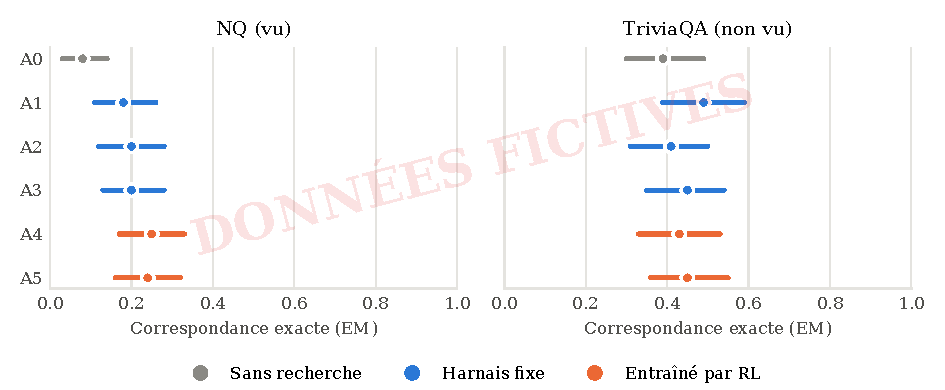
\includegraphics[width=\linewidth]{genere/fig_em.pdf}
\caption{Précision des six systèmes selon le jeu de questions. Données : run d'évaluation du 9 novembre 2026 sur Kaggle (version 4 du kernel). Une observation = une question traitée par un système ; effectif : 100 questions par jeu et par système, aucune écartée (les sorties sans réponse comptent comme fausses). Le point est l'EM moyen, le trait son intervalle bootstrap à 95~\% (1\,000 rééchantillonnages).}
\label{fig:em}
\end{figure}

\subsection{Tests des hypothèses}
Le tableau~\ref{tab:tests} applique les règles de décision fixées avant le run (tableau~\ref{tab:test}).

\begin{table}[ht]
\centering\small
\begin{tabular}{@{}lp{7.6cm}l@{}}
\toprule
Hyp. & Résultat du test & Verdict\\
\midrule
HA1 & Écarts d'EM RL $-$ harnais, NQ et TriviaQA réunis (200 questions) : A4--A1 10{,}0 pt ($p_{\text{Holm}}$ $<$\,0{,}001); A4--A2 14{,}5 pt ($p_{\text{Holm}}$ $<$\,0{,}001); A4--A3 12{,}5 pt ($p_{\text{Holm}}$ $<$\,0{,}001); A5--A1 12{,}5 pt ($p_{\text{Holm}}$ $<$\,0{,}001); A5--A2 17{,}0 pt ($p_{\text{Holm}}$ $<$\,0{,}001); A5--A3 15{,}0 pt ($p_{\text{Holm}}$ $<$\,0{,}001). 6 paire(s) sur 6 positives et significatives. & soutenue\\
HA2 & Écart RL $-$ harnais : 12{,}8 pt sur NQ, 14{,}3 pt sur TriviaQA ; différence $-$1{,}5 pt [$-$10{,}8\,; 7{,}3]. & non soutenue\\
HA3a & Recherches par question, RL $-$ A2 : 0{,}92 [0{,}79\,; 1{,}05], 200 questions. & soutenue\\
HA3b & Même écart, questions où A0 répond juste : 0{,}74 [0{,}48\,; 0{,}98], 44 questions. & soutenue\\
\bottomrule
\end{tabular}

\caption{Résultat des tests. Écarts d'EM en points de pourcentage, écarts de recherches en nombre de recherches par question ; entre crochets, intervalle bootstrap à 95~\%.\iffictif\ \textcolor{red}{Valeurs fictives.}\fi}
\label{tab:tests}
\end{table}

\paragraph{HA1 (\valHA{HA1}{verdict}\fictif).} Les six écarts entre agents entraînés et harnais sont positifs, de 10 à 17 points d'EM sur les 200 questions, et tous restent significatifs après correction de Holm ($p < 0{,}001$). Ces écarts sont dans la zone où la simulation de la section~\ref{sec:methode} donnait une puissance d'au moins une chance sur deux : l'expérience pouvait les voir.

\paragraph{HA2 (\valHA{HA2}{verdict}\fictif).} L'avance des agents entraînés est de \valHA{HA2}{ecart_nq}~points sur NQ, vu à l'entraînement, et de \valHA{HA2}{ecart_tqa}~points sur TriviaQA, non vu. La différence, \valHA{HA2}{d}~point, va à l'inverse de l'hypothèse, et son intervalle [\valHA{HA2}{lo}\,; \valHA{HA2}{hi}] contient zéro. L'avantage des agents ne se limite donc pas au jeu vu ; un écart modeste entre les deux jeux resterait toutefois indétectable avec 100 questions par jeu.

\paragraph{HA3a (\valHA{HA3a}{verdict}\fictif).} Les agents entraînés font en moyenne \valHA{HA3a}{d} recherche de plus par question que ReAct, avec un intervalle de [\valHA{HA3a}{lo}\,; \valHA{HA3a}{hi}] sur \valHA{HA3a}{n} questions. Aucun des deux ne répond jamais sans chercher, alors que ReAct le fait sur \valSansRech{A2}~\% des questions. La figure~\ref{fig:cout} nuance ce coût : A5 atteint une précision voisine de celle de A4, et meilleure sur TriviaQA, avec environ une recherche de moins par question que A4 et presque deux de moins que IRCoT.

\paragraph{HA3b (\valHA{HA3b}{verdict}\fictif).} Sur les \valHA{HA3b}{n} questions auxquelles A0 répond juste, l'écart avec ReAct reste de \valHA{HA3b}{d} recherche par question [\valHA{HA3b}{lo}\,; \valHA{HA3b}{hi}]. Sur ces questions, ni les agents ni ReAct ne s'abstiennent de chercher.

\begin{figure}[ht]
\centering
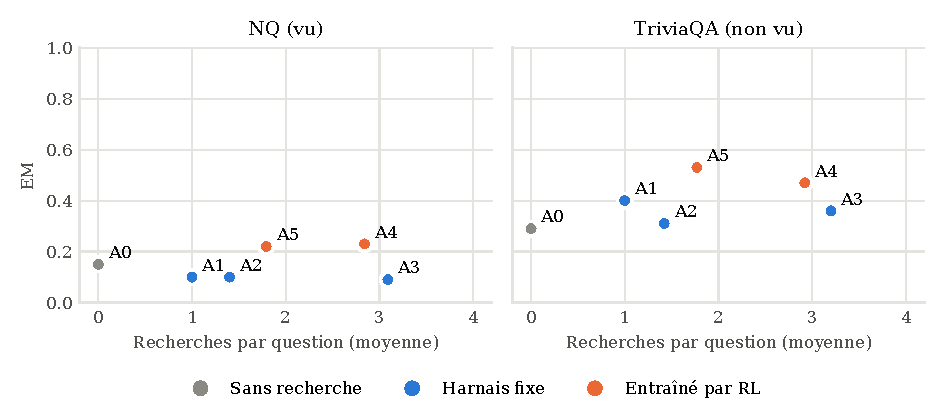
\includegraphics[width=\linewidth]{genere/fig_cout.pdf}
\caption{Précision et coût. Chaque point est un système : en abscisse, le nombre moyen de recherches par question ; en ordonnée, l'EM. Mêmes données et mêmes effectifs que la figure~\ref{fig:em}. Un système placé plus haut et plus à gauche obtient plus avec moins de recherches.}
\label{fig:cout}
\end{figure}


\subsection{Où se joue l'avantage : analyses exploratoires}\label{sec:exploratoire}
Les analyses de cette section n'étaient pas prévues dans le plan d'analyse : elles ont été choisies après avoir vu les résultats, et ne portent aucun verdict. Elles décomposent l'avantage des agents selon les trois moments d'une recherche : trouver l'information, la lire, et répondre quand elle manque. Une réponse est dite « dans les passages » quand une des réponses attendues, normalisée comme pour l'EM, apparaît telle quelle dans un passage lu ; c'est une estimation, car un passage peut contenir la chaîne sans la justifier.

\paragraph{Ce que la recherche fait gagner et perdre.} Comparée au modèle seul, question par question, la recherche ne fait pas qu'ajouter des bonnes réponses : elle en retire aussi (figure~\ref{fig:transitions}). Les trois harnais gagnent de \valAp{A2-gagnees} à \valAp{A3-gagnees} questions mais en perdent presque autant, de \valAp{A1-perdues} à \valAp{A3-perdues} ; leur bilan est presque nul. Les agents entraînés gagnent davantage (\valAp{A4-gagnees} et \valAp{A5-gagnees}) et perdent peu (\valAp{A4-perdues} et \valAp{A5-perdues}). Les trajectoires des harnais montrent des réponses reprises d'un passage voisin mais hors sujet : à la question de l'entrée du half-pipe à ski aux Jeux olympiques (2014), le RAG répond « 1998 », date tirée d'un passage sur le snowboard ; à la question du lieu où sont absorbés la plupart des nutriments (« small intestine »), il répond « jejunum and ileum », repris d'un passage sur le duodénum. Le modèle seul répondait juste dans les deux cas.

\begin{figure}[ht]
\centering
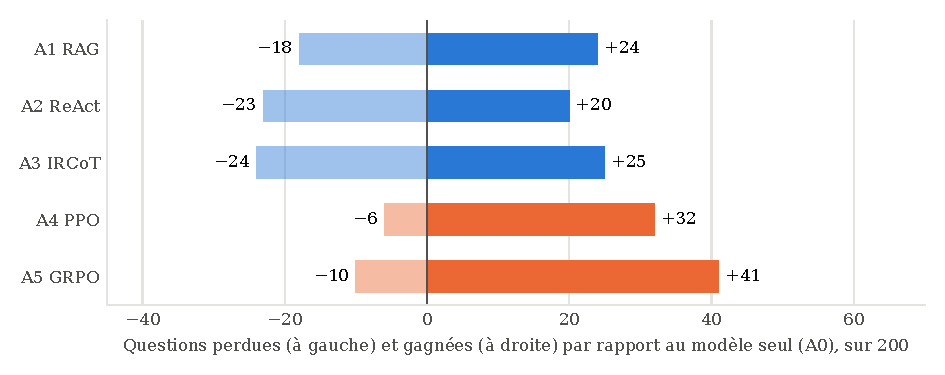
\includegraphics[width=\linewidth]{genere/fig_transitions.pdf}
\caption{Ce que la recherche fait gagner et perdre par rapport au modèle seul. À droite, les questions que A0 rate et que le système réussit ; à gauche, celles que A0 réussit et que le système rate. 200 questions (NQ et TriviaQA réunis), une barre par système.}
\label{fig:transitions}
\end{figure}

\paragraph{Trouver ou lire.} La figure~\ref{fig:decomposition} sépare les deux moments. Les systèmes trouvent la réponse à peu près aussi souvent : elle figure dans les passages lus pour \valAp{harnais-trouvee}~\% des trajectoires des harnais et \valAp{rl-trouvee}~\% de celles des agents. Ils diffèrent surtout dans ce qu'ils en font : quand la réponse est dans les passages, les harnais la donnent dans \valAp{harnais-em_t}~\% des cas, les agents dans \valAp{rl-em_t}~\% ; quand elle n'y est pas, les agents répondent encore juste dans \valAp{rl-em_nt}~\% des cas, contre \valAp{harnais-em_nt}~\% pour les harnais (figure~\ref{fig:arbre}).

Une décomposition contrefactuelle chiffre ces trois contributions. L'écart moyen d'EM entre agents et harnais, \valAp{ox-total}~points [\valAp{ox-total-lo}\,; \valAp{ox-total-hi}], s'écrit exactement comme la somme de trois termes : trouver plus souvent la réponse, \valAp{ox-trouver}~points [\valAp{ox-trouver-lo}\,; \valAp{ox-trouver-hi}], soit \valAp{ox-trouver-part}~\% de l'écart ; mieux la lire quand elle est là, \valAp{ox-lire}~points [\valAp{ox-lire-lo}\,; \valAp{ox-lire-hi}], soit \valAp{ox-lire-part}~\% ; mieux répondre quand elle manque, \valAp{ox-sans}~points [\valAp{ox-sans-lo}\,; \valAp{ox-sans-hi}], soit \valAp{ox-sans-part}~\%. Les intervalles sont obtenus par bootstrap sur les questions. L'essentiel de l'avantage se joue donc après la recherche, non pendant.

\begin{figure}[ht]
\centering
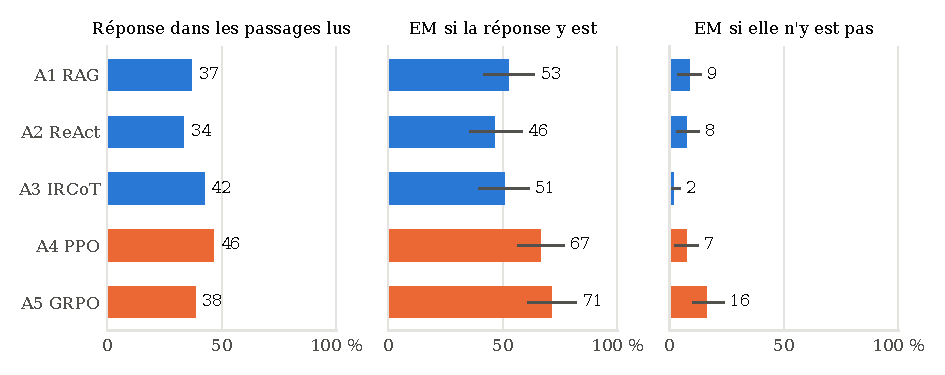
\includegraphics[width=\linewidth]{genere/fig_decomposition.pdf}
\caption{Trouver ou lire. À gauche, part des questions où la réponse attendue figure dans les passages lus ; au centre et à droite, EM selon que la réponse y figure ou non, avec son intervalle bootstrap à 95~\%. 200 questions par système ; effectifs de chaque cas dans \texttt{analysis/analyse\_approfondie.py}.}
\label{fig:decomposition}
\end{figure}

\begin{figure}[ht]
\centering
\begin{tikzpicture}[scale=0.92, every node/.style={transform shape},
  q/.style={draw, rounded corners, align=center, fill=gray!10, minimum height=0.9cm, font=\small},
  n/.style={draw, rounded corners, align=center, minimum width=3.6cm, minimum height=1cm, font=\small, fill=white},
  f/.style={draw, rounded corners, align=center, minimum width=3.4cm, minimum height=1cm, font=\small, fill=green!8},
  >={Stealth[length=2.2mm]}]
  \node[q] (r) at (0,0) {Une question,\\ un système qui cherche};
  \node[n] (t) at (4.6,1.4) {Réponse dans\\ les passages lus\\ {\footnotesize\textcolor{blue!70!black}{H \valAp{harnais-trouvee}\,\%} \quad \textcolor{orange!80!black}{RL \valAp{rl-trouvee}\,\%}}};
  \node[n] (nt) at (4.6,-1.4) {Réponse absente\\ des passages\\ {\footnotesize (le reste des trajectoires)}};
  \node[f] (tj) at (9.6,1.4) {Réponse juste\\ {\footnotesize\textcolor{blue!70!black}{H \valAp{harnais-em_t}\,\%} \quad \textcolor{orange!80!black}{RL \valAp{rl-em_t}\,\%}}};
  \node[f] (ntj) at (9.6,-1.4) {Réponse juste\\ {\footnotesize\textcolor{blue!70!black}{H \valAp{harnais-em_nt}\,\%} \quad \textcolor{orange!80!black}{RL \valAp{rl-em_nt}\,\%}}};
  \draw[->, thick] (r) -- node[above, sloped, font=\footnotesize, align=center] {trouver\\ +\valAp{ox-trouver} pt (\valAp{ox-trouver-part}\,\%)} (t);
  \draw[->, thick] (r) -- (nt);
  \draw[->, thick] (t) -- node[above, font=\footnotesize] {lire} (tj);
  \draw[->, thick] (nt) -- node[below, font=\footnotesize] {sans appui} (ntj);
  \node[font=\footnotesize, align=left, anchor=west] at (11.5,1.4) {+\valAp{ox-lire} pt\\ (\valAp{ox-lire-part}\,\%)};
  \node[font=\footnotesize, align=left, anchor=west] at (11.5,-1.4) {+\valAp{ox-sans} pt\\ (\valAp{ox-sans-part}\,\%)};
\end{tikzpicture}
\caption{Arbre de décomposition de l'avantage des agents. Pour chaque moment de la recherche : la proportion observée pour les harnais (H, en bleu, A1 à A3 réunis, 600 trajectoires) et pour les agents entraînés (RL, en orange, A4 et A5, 400 trajectoires), puis, à droite, la part de l'écart d'EM qui s'y joue d'après la décomposition contrefactuelle.}
\label{fig:arbre}
\end{figure}

\paragraph{Quoi chercher.} Le tableau~\ref{tab:requetes} décrit les requêtes. La première requête trouve la réponse aussi souvent pour tous les systèmes qui cherchent, autour d'un tiers des questions (de \valAp{A2-trouvee1} à \valAp{A1-trouvee1}~\%), et les agents ne formulent pas de meilleures premières requêtes : A5 recopie la question dans \valAp{A5-copie1}~\% des cas, A4 dans \valAp{A4-copie1}~\%. Leurs recherches suivantes ajoutent peu : elles font trouver la réponse sur \valAp{A4-reform}~\% des questions de plus pour A4 et \valAp{A5-reform}~\% pour A5, et une question sur quatre environ contient une requête répétée mot pour mot (\valAp{A4-repetees}~\% pour A4, \valAp{A5-repetees}~\% pour A5). Une part du surcoût mesuré par HA3a est donc un gaspillage au sens strict. En jetons générés, en revanche, agents et harnais itératifs coûtent à peu près autant (environ \valAp{A2-jetons} jetons pour ReAct, \valAp{A5-jetons} pour A5).

\begin{table}[ht]
\centering\small
\begin{tabular}{@{}lcccccc@{}}
\toprule
Système & Mots par & Recouvrement & 1\textsuperscript{re} requête & Requêtes & Requête & Jetons\\
 & requête & avec la question & = question & distinctes & répétée & générés\\
\midrule
A1 RAG & 12{,}4 & 1{,}00 & 100\,\% & 1{,}0 & 0\,\% & 13\\
A2 ReAct & 6{,}2 & 0{,}42 & 4\,\% & 1{,}3 & 6\,\% & 151\\
A3 IRCoT & 14{,}5 & 0{,}45 & 100\,\% & 3{,}1 & 0\,\% & 139\\
\midrule
A4 PPO & 8{,}2 & 0{,}50 & 70\,\% & 2{,}6 & 29\,\% & 162\\
A5 GRPO & 12{,}0 & 0{,}85 & 90\,\% & 1{,}5 & 26\,\% & 166\\
\bottomrule
\end{tabular}

\caption{Les requêtes émises, sur 200 questions. Recouvrement : indice de Jaccard entre les mots de la requête et ceux de la question (1 = mêmes mots). Requête répétée : part des questions où une même requête est émise deux fois. Jetons : nombre moyen de jetons générés par question.}
\label{tab:requetes}
\end{table}

\paragraph{Typologie des erreurs.} La figure~\ref{fig:erreurs} classe automatiquement chaque réponse fausse en quatre types. L'absence de la réponse dans les passages domine pour tous les systèmes : c'est la limite du corpus réduit. Deux types distinguent pourtant les familles. Les harnais laissent passer la bonne réponse sous leurs yeux (de \valAp{A1-err2} à \valAp{A3-err2} questions), deux à trois fois plus souvent que A5 (\valAp{A5-err2}). IRCoT ne répond pas du tout sur \valAp{A3-err0} questions, surtout par abstention. Les agents, eux, ont plus de réponses proches mais mal formulées (\valAp{A4-err1} et \valAp{A5-err1}, F1 au moins 0,5), comme « Dame Judi Dench » pour « Judi Dench » : la correspondance exacte les pénalise un peu.

\begin{figure}[ht]
\centering
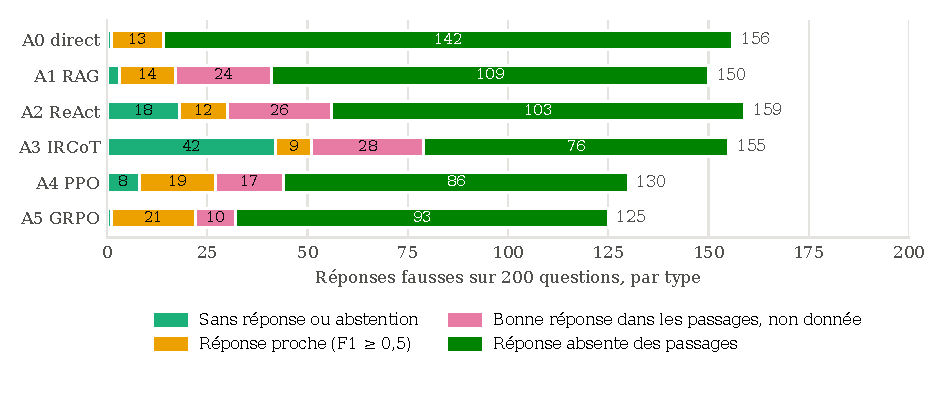
\includegraphics[width=\linewidth]{genere/fig_erreurs.pdf}
\caption{Typologie automatique des réponses fausses, sur 200 questions par système. Sans réponse : sortie sans réponse exploitable ou abstention explicite. Réponse proche : F1 d'au moins 0,5 avec une réponse attendue. Bonne réponse dans les passages : réponse fausse alors qu'une réponse attendue figurait dans un passage lu. Réponse absente : ni l'un ni l'autre.}
\label{fig:erreurs}
\end{figure}

\paragraph{Toutes les comparaisons.} La figure~\ref{fig:matrice} donne l'écart d'EM pour les quinze paires de systèmes. Elle fait apparaître deux blocs : entre eux, les quatre systèmes non entraînés (réponse directe et trois harnais) ne se distinguent pas ; les deux agents dominent chacun de ces quatre systèmes ; entre eux, A4 et A5 ne se distinguent pas.

\begin{figure}[ht]
\centering
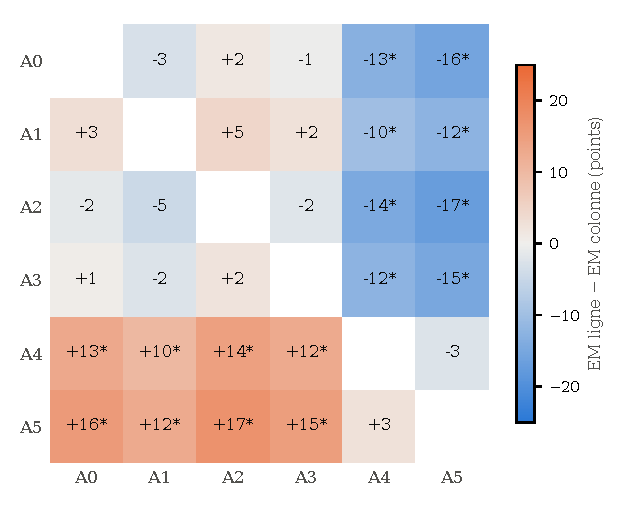
\includegraphics[width=0.62\linewidth]{genere/fig_matrice.pdf}
\caption{Écart d'EM entre chaque paire de systèmes (ligne moins colonne, en points), sur les 200 questions. Orange : la ligne fait mieux ; bleu : la colonne fait mieux. Astérisque : test de McNemar significatif au seuil de 5~\% avec correction de Bonferroni pour les 15 paires. Analyse descriptive, hors du plan d'analyse.}
\label{fig:matrice}
\end{figure}


\subsection{Robustesse et analyses avancées}\label{sec:avance}
Ces analyses, elles aussi exploratoires, répondent à cinq objections que l'on peut faire aux résultats précédents.

\paragraph{L'écart vient-il seulement de questions plus faciles ?} Un modèle de régression logistique explique la réussite de chaque trajectoire (\valAv{glm-nobs} trajectoires des cinq systèmes qui cherchent, \valAv{glm-nq} questions) par la famille du système, la présence de la réponse dans les passages, leur interaction, la connaissance préalable de la question et le jeu ; les erreurs-types sont groupées par question, puisque chaque question apparaît cinq fois (tableau~\ref{tab:glm}). À situation égale, être un agent entraîné multiplie les chances de bonne réponse par \valAv{glm-rl} [\valAv{glm-rl-lo}\,; \valAv{glm-rl-hi}]. L'avantage des agents ne s'explique donc ni par la difficulté des questions, ni par des passages plus utiles. L'interaction entre famille et présence de la réponse est en revanche nulle (\valAv{glm-rlxtrouvee}, $p = \valAv{glm-rlxtrouvee-p}$) : en chances relatives, l'avantage des agents est le même que la réponse soit dans les passages ou non. La part importante de la « lecture » dans la décomposition additive (section~\ref{sec:exploratoire}) tient au fait que, quand la réponse est là, il y a plus de points à gagner ; ce que les agents font mieux, c'est répondre à partir de l'information dont ils disposent, qu'elle vienne des passages ou de leurs connaissances.

\begin{table}[ht]
\centering\small
\begin{tabular}{@{}lccc@{}}
\toprule
Variable & Odds ratio & IC 95\,\% & $p$\\
\midrule
Agent entraîné (RL) & 2{,}62 & [1{,}44\,; 4{,}78] & 0{,}002\\
Réponse dans les passages & 12{,}96 & [6{,}91\,; 24{,}31] & $<$\,0{,}001\\
RL $\times$ réponse dans les passages & 1{,}03 & [0{,}50\,; 2{,}12] & 0{,}942\\
Question connue du modèle seul (A0 juste) & 5{,}61 & [2{,}87\,; 10{,}97] & $<$\,0{,}001\\
Jeu TriviaQA (contre NQ) & 3{,}90 & [2{,}19\,; 6{,}96] & $<$\,0{,}001\\
\bottomrule
\end{tabular}

\caption{Régression logistique de la réussite (EM) sur 1\,000 trajectoires (A1 à A5, 200 questions), erreurs-types groupées par question. Un odds ratio supérieur à 1 signifie de meilleures chances de réussite. Référence : harnais, réponse absente des passages, question non connue, jeu NQ.}
\label{tab:glm}
\end{table}

\paragraph{Les recherches supplémentaires rapportent-elles ?} La figure~\ref{fig:fourragement} trace, pour chaque système, la part des questions dont la réponse a été trouvée après $k$ recherches, et ce qu'apporte chaque recherche. Le rendement décroît brutalement : la première recherche trouve la réponse pour environ un tiers des questions ; la deuxième n'ajoute que de \valAv{A5-marg2} à \valAv{A3-marg2}~points, sauf pour A4 (\valAv{A4-marg2}~points) ; la troisième et la quatrième presque rien. Pourtant, IRCoT fait au moins trois recherches sur \valAv{A3-atteint3}~\% des questions et A4 sur \valAv{A4-atteint3}~\%. C'est la courbe de rendement décroissant que décrit la théorie du fourragement, et un agent qui la suivrait s'arrêterait après la deuxième recherche ; sans coût dans sa récompense, A4 continue.

\begin{figure}[ht]
\centering
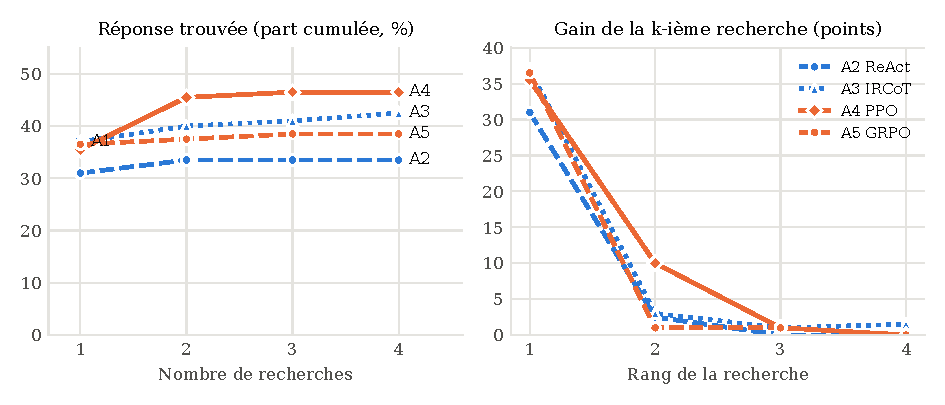
\includegraphics[width=\linewidth]{genere/fig_fourragement.pdf}
\caption{Rendement des recherches successives. À gauche, part cumulée des questions où la réponse attendue figure dans les passages lus après $k$ recherches ; à droite, gain apporté par la $k$-ième recherche, en points. 200 questions par système ; une question qui s'arrête avant la $k$-ième recherche n'apporte aucun gain à ce rang. A1 ne fait qu'une recherche.}
\label{fig:fourragement}
\end{figure}

\paragraph{Le résultat dépend-il de la métrique ?} La correspondance exacte compte faux « Dame Judi Dench » pour « Judi Dench ». Le tableau~\ref{tab:sensibilite} recalcule l'écart entre agents et harnais avec une correspondance souple (une réponse attendue apparaît, en mots entiers, dans la réponse donnée) et avec F1. L'écart reste du même ordre (\valAv{sens-souple}~points en correspondance souple, \valAv{sens-f1} en F1), et les six comparaisons restent significatives après correction de Holm. Les tailles d'effet sont grandes : pour chaque paire, les questions que seul l'agent réussit sont \valAv{or-min} à \valAv{or-max} fois plus nombreuses que celles que seul le harnais réussit.

\begin{table}[ht]
\centering\small
\begin{tabular}{@{}lcc@{}}
\toprule
Métrique & Écart RL $-$ harnais [IC 95\,\%] & Paires significatives (Holm)\\
\midrule
Correspondance exacte (EM) & 13{,}6 pt [9{,}2\,; 18{,}2] & 6 sur 6\\
Correspondance souple & 12{,}5 pt [8{,}1\,; 17{,}2] & 6 sur 6\\
F1 & 15{,}5 pt [11{,}3\,; 19{,}9] & —\\
\midrule
\multicolumn{3}{@{}l}{\emph{Tailles d'effet (EM) : odds ratio de McNemar, questions réussies par le seul agent / par le seul harnais}}\\
A4 contre A1 & OR = 4{,}3 [1{,}7\,; 12{,}9] & 26 contre 6 questions\\
A4 contre A2 & OR = 4{,}6 [2{,}1\,; 11{,}5] & 37 contre 8 questions\\
A4 contre A3 & OR = 3{,}8 [1{,}8\,; 9{,}0] & 34 contre 9 questions\\
A5 contre A1 & OR = 6{,}0 [2{,}3\,; 19{,}8] & 30 contre 5 questions\\
A5 contre A2 & OR = 5{,}2 [2{,}4\,; 12{,}9] & 42 contre 8 questions\\
A5 contre A3 & OR = 5{,}3 [2{,}3\,; 14{,}1] & 37 contre 7 questions\\
\bottomrule
\end{tabular}

\caption{Sensibilité de HA1 à la métrique, et tailles d'effet. Écart moyen entre agents (A4, A5) et harnais (A1 à A3) sur 200 questions, intervalle bootstrap apparié. Odds ratio de McNemar avec intervalle exact.}
\label{tab:sensibilite}
\end{table}

\paragraph{La décomposition tient-elle sur chaque jeu ?} Recalculée sur chaque jeu séparément (tableau~\ref{tab:jeux}), la part « trouver » reste faible sur les deux. Sur NQ, où le corpus couvre moins bien les réponses, l'écart se joue presque autant sans appui (\valAv{jeu-nq-sans}~points) qu'à la lecture (\valAv{jeu-nq-lire}) ; sur TriviaQA, surtout à la lecture (\valAv{jeu-triviaqa-lire}~points). Les intervalles, sur 100 questions, sont larges.

\begin{table}[ht]
\centering\small
\begin{tabular}{@{}lcccc@{}}
\toprule
Jeu & Trouver & Lire & Sans appui & Écart total\\
\midrule
NQ (vu) & 1{,}2 [0{,}3\,; 2{,}7] & 6{,}5 [2{,}2\,; 11{,}0] & 5{,}1 [1{,}9\,; 9{,}0] & 12{,}8 [7{,}2\,; 18{,}8]\\
TriviaQA (non vu) & 2{,}7 [0{,}5\,; 5{,}1] & 9{,}7 [4{,}7\,; 15{,}1] & 2{,}0 [$-$2{,}0\,; 6{,}3] & 14{,}3 [7{,}7\,; 20{,}8]\\
\bottomrule
\end{tabular}

\caption{Décomposition de l'écart d'EM entre agents et harnais, jeu par jeu, en points ; intervalle bootstrap à 95~\% sur les 100 questions du jeu.}
\label{tab:jeux}
\end{table}

\paragraph{Les systèmes réussissent-ils les mêmes questions ?} Les deux agents se ressemblent davantage entre eux (indice de Jaccard de \valAv{comp-jac_rl} entre leurs ensembles de questions réussies) que les harnais entre eux (\valAv{comp-jac_h} en moyenne). Une question réussie par au moins un harnais l'est dans \valAv{comp-oracle_h}~\% des cas, par au moins un agent dans \valAv{comp-oracle_rl}~\%, par au moins un des six systèmes dans \valAv{comp-oracle_tous}~\% : aucun système ne trouve la réponse à \valAv{comp-aucun}~\% des questions. Ce plafond est d'abord celui du corpus réduit.

\FloatBarrier
\section{Discussion}\label{sec:discussion}
% Cinq mouvements (étape 10) : rappel, comparaison, explication, contributions, limites et ouverture.

\fictifnote{Cette discussion commente des résultats fictifs.}

\subsection{Rappel des résultats}
À corpus, retriever, budget et questions identiques, les agents entraînés par renforcement répondent nettement mieux que les harnais fixes, sur le jeu vu comme sur le jeu non vu. Ils ne doivent cet avantage ni à une recherche plus sobre ni à de meilleures requêtes : ils cherchent à chaque question, souvent en recopiant la question, plus souvent que ReAct, y compris quand le modèle connaît déjà la réponse. Ce qui les distingue, c'est qu'une recherche les égare beaucoup moins.

\subsection{Comparaison avec la littérature}
Nos résultats confirment le sens du gain rapporté par les auteurs de Search-R1 \citep{jin2025search}, cette fois face à des harnais qui partagent le corpus, le retriever et le budget de l'agent : le gain subsiste quand ces trois conditions sont communes, même si les poids du modèle, eux, diffèrent. Ils nuancent en revanche l'idée d'un avantage limité aux jeux d'entraînement. Un contrôleur appris sur HotpotQA perd en qualité de réponse sur MuSiQue \citep{raikote2026policy} ; ici, l'avance est aussi forte sur TriviaQA que sur NQ. Les deux jeux sont toutefois proches (questions factuelles à une étape) : notre « non vu » est un changement de distribution modeste. Sur le coût, nos agents confirment le constat de surrecherche \citep{wu2025search,tang2026saas} : ils ne se passent jamais de chercher. Enfin, les pertes des harnais rejoignent les travaux qui montrent qu'un modèle se laisse distraire par des passages non pertinents \citep{yoran2023making} et que la recherche peut nuire sur ce que le modèle sait déjà \citep{mallen2022when,maekawa2024retrieval}.

\subsection{Explication}
Le cadre du fourragement de l'information (section~\ref{sec:cadre}) distingue deux choses : décider s'il faut fourrager et quand s'arrêter, et tirer parti de ce que l'on trouve. Nos résultats séparent les deux. Sur la décision, le cadre rend compte de ce que l'on observe sans le distinguer des harnais : la récompense de Search-R1 ne fait payer aucune recherche, et les agents cherchent toujours, même quand le gain attendu est faible (HA3a, HA3b) ; mais ReAct, sur les questions que le modèle connaît, ne renonce pas davantage à chercher. La surrecherche n'est donc pas propre aux agents entraînés ; ils cherchent seulement plus. La courbe de gain des recherches (figure~\ref{fig:fourragement}) en donne la mesure la plus directe : au-delà de la deuxième recherche, le gain est presque nul pour tous les systèmes, et un fourrageur qui comparerait ce gain à un coût s'arrêterait là ; IRCoT, par règle, et A4, faute de coût, ne s'arrêtent pas. Leur avantage se situe ailleurs, du côté de l'exploitation : ce sont des fourrageurs qui ne choisissent pas mieux leurs parcelles, mais qui tirent mieux parti de ce qu'ils y trouvent. Les analyses exploratoires de la section~\ref{sec:exploratoire} le chiffrent : leurs premières requêtes trouvent la réponse aussi souvent que celles des harnais, et la plus grande part de l'écart (\valAp{ox-lire-part}~\%) tient à ce qu'ils font d'une réponse présente dans les passages ; un quart tient à ce qu'ils répondent mieux quand elle manque. Le modèle logistique (section~\ref{sec:avance}) précise cette lecture : en chances relatives, l'avantage des agents est le même avec ou sans la réponse dans les passages. Ils ne lisent donc pas mieux au sens étroit ; ils répondent mieux à partir de l'information dont ils disposent, et se laissent moins détourner de ce qu'ils savent par un passage trompeur. Une lecture compatible avec nos données est que le renforcement, qui ne récompense que la bonne réponse finale, pénalise indirectement l'usage d'un passage trompeur ; le modèle Instruct, lui, reprend des passages voisins mais hors sujet alors même que son prompt l'autorise à s'en remettre à ses connaissances. Sur NQ, où le corpus ne contient la réponse que pour une question sur quatre, cette tendance coûte plus que la recherche ne rapporte. Ces chiffres décrivent où se joue l'écart ; ils n'en établissent pas la cause, et la mesure de « réponse présente » est une estimation par chaîne de caractères.

\emph{Explications concurrentes.} Deux autres lectures sont possibles, et notre protocole ne permet pas de les écarter. La première tient au corpus : A4 et A5 ont été entraînés avec E5 sur Wikipédia 2018, la source de notre sous-corpus ; ils connaissent le format et le bruit de ces passages, ce que n'apprennent pas les harnais. La seconde tient au modèle : les agents partent du modèle de base, les harnais du modèle Instruct, dont l'ajustement aux consignes pourrait renforcer la déférence envers le contexte. Comparer A4 et A5 aux agents Search-R1 issus de la version Instruct, et faire varier le retriever (H4), permettra de départager ces lectures dans le mémoire.

\subsection{Contributions}
\textbf{Théorique.} L'étude montre, sur un agent de recherche, la courbe de rendement décroissant que prédit la théorie du fourragement, et l'absence de la règle d'arrêt qui devrait l'accompagner quand la récompense ignore le coût. Elle sépare aussi trois composantes que la littérature confond souvent sous « savoir chercher » : la décision de chercher, le choix de la requête, et l'usage de ce qui est trouvé ; elle propose une décomposition simple de la précision selon ces moments, réutilisable pour d'autres agents. Dans nos conditions, les agents entraînés se distinguent par la seconde et non par la première, ce qui est compatible avec un cadre de fourragement où la récompense ignore le coût. La question « quand chercher ? » reste donc ouverte même pour les agents entraînés.

\textbf{Pratique.} Trois recommandations, chacune pour un acteur précis. L'équipe qui ajoute un moteur de recherche à un petit modèle Instruct devrait d'abord comparer, sur un échantillon de ses questions, le modèle seul et le modèle avec recherche : sur NQ, la recherche a fait baisser la précision de nos trois harnais. Celle qui dispose d'un agent Search-R1 public et d'un corpus encyclopédique proche de Wikipédia peut en attendre, dans des conditions comparables aux nôtres, un gain de précision pour environ une recherche de plus par question qu'un ReAct ; sur un autre corpus, ce gain reste à vérifier. Enfin, l'équipe qui entraîne un agent devrait ajouter un coût par recherche à sa récompense : sans lui, l'agent ne renonce jamais à chercher, même sur ce qu'il sait ; c'est l'hypothèse H3 du mémoire.

\subsection{Limites et pistes}
Ces limites valent quels que soient les résultats. Le tableau~\ref{tab:validite} les range selon le type de validité qu'elles menacent.

\begin{table}[ht]
\centering\small
\begin{tabular}{@{}p{2.1cm}p{5.2cm}p{6.6cm}@{}}
\toprule
Validité & Menace & Ce qui a été fait, ce qui reste\\
\midrule
Interne & A0 à A3 utilisent Qwen2.5-3B-Instruct, A4 et A5 un modèle entraîné à partir de Qwen2.5-3B (base) : l'écart mélange règle de recherche et modèle. & Même famille, même taille, même budget. Les agents issus de la version Instruct permettront de séparer les deux dans le mémoire.\\
Interne & Les prompts de A2 et A3 ont été corrigés en mise au point. & Correction faite sur d'autres questions (graine 7), puis gel. A3 s'abstient explicitement sur \valAbst{A3} des 200 questions d'évaluation : il est probablement sous-estimé.\\
Construit & L'EM compte comme fausses des réponses justes formulées autrement. & F1 rapporté à côté de l'EM ; même normalisation que Search-R1 pour tous.\\
Construit & La connaissance préalable est mesurée par une seule réponse de A0, produite par le modèle Instruct. & Le mémoire prévoit huit échantillons par question (oracle de connaissance).\\
Statistique & 100 questions par jeu, une graine : un vrai écart de 10 points n'a qu'environ \valPuiss{200}{10}{holm} de chances d'être détecté pour HA1. & Règles fixées d'avance, correction de Holm, intervalles rapportés. Une absence d'effet significatif ne prouve pas l'absence d'effet. Le mémoire passe à 500 questions par jeu.\\
Statistique & Décodage glouton : la répétabilité exacte de la génération entre deux machines n'est pas testée. & La recherche est rendue déterministe (ex aequo départagés) ; la génération reste à tester.\\
Externe & Corpus d'un million de passages : réponse dans les trois premiers passages pour 25~\% (NQ) et 44~\% (TriviaQA) des questions ; A4 et A5 ont été entraînés sur le corpus complet. & Couverture mesurée et rapportée. Le plafond de précision est bas pour tous les systèmes qui cherchent.\\
Externe & Deux jeux à une étape, en anglais, Wikipédia 2018, modèles de 3 milliards de paramètres. & Les jeux multi-étapes et d'autres retrievers sont prévus dans le mémoire (H4).\\
\bottomrule
\end{tabular}
\caption{Menaces à la validité. Interne : l'écart vient-il bien de la règle de recherche ? Construit : mesure-t-on ce que l'on croit mesurer ? Statistique : l'échantillon permet-il de conclure ? Externe : le résultat vaut-il ailleurs ?}
\label{tab:validite}
\end{table}

\noindent\textbf{Causalité.} Nous comparons des systèmes complets : aucun écart ne peut être attribué à un seul facteur. L'analyse des questions perdues après recherche, non prévue dans le plan, reste exploratoire.

\textbf{Pistes.} La limite principale, des modèles de départ différents, peut être levée : les auteurs de Search-R1 publient aussi des points de contrôle entraînés à partir de Qwen2.5-3B-Instruct (\texttt{SearchR1-nq\_hotpotqa\_train-qwen2.5-3b-it-em-\{ppo,grpo\}-v0.3}), que l'on peut comparer à leur propre modèle de départ. Cette comparaison appariée permet de poser la question du débat de la section~\ref{sec:revue} : le renforcement élargit-il ce que l'agent finit par résoudre, ou le rend-il seulement plus fiable ? Elle se mesure par pass@k sur des tirages multiples, avec l'inférence appariée de \citet{yang2026crossovers}, dans un environnement où la réponse est toujours atteignable ; c'est l'objet de la suite du mémoire. Deux autres hypothèses ne sont pas testées ici : une pénalité par recherche dans la récompense réduit-elle le nombre d'appels sans perte forte de précision (entraînement GRPO à petite échelle), et un changement de retriever dégrade-t-il plus les agents entraînés que les harnais fixes ? Une analyse qualitative des échecs sur des trajectoires annotées compléterait la mesure : le mémoire prévoit d'en annoter 100 à la main et d'en faire classer 300 par un juge automatique, avec un accord mesuré par le kappa de Cohen.

\FloatBarrier
\section{Conclusion}\label{sec:conclusion}
\fictifnote{Conclusion écrite sur les résultats fictifs.}
Nous avons comparé, à corpus, retriever, budget et questions identiques, deux agents de recherche entraînés par renforcement et quatre systèmes à règle fixe. Les agents entraînés répondent nettement mieux, sur le jeu vu comme sur le jeu non vu. Mais ils ne cherchent pas mieux au sens où on l'entend d'habitude : ils cherchent toujours, davantage que ReAct, y compris quand le modèle sait déjà répondre. Leur avantage tient à l'usage des passages : la plus grande part de l'écart se joue une fois la réponse sous leurs yeux, et une recherche les égare moins. Le cadre du fourragement de l'information rend compte des deux faits : sans coût dans la récompense, rien n'incite l'agent à s'arrêter ; une récompense sur la seule réponse finale peut, en revanche, l'avoir conduit à écarter l'information trompeuse, ce que nos données suggèrent sans l'établir. Ces conclusions valent pour un petit corpus, un petit modèle et deux jeux de questions proches. Le mémoire les mettra à l'épreuve sur sept jeux, en testant une pénalité par recherche (H3) et un changement de retriever (H4).



\chapter{Le renforcement élargit-il ce que l'agent sait faire ?}\label{ch:partie2}
% Fichier généré par scripts/assemble_memoire.py : ne pas modifier à la main.
\section{Question et lien avec la partie 1}

La partie 1 a montré qu'à corpus et questions identiques, les agents Search-R1 battent les harnais fixes au premier essai, et que l'avantage se joue à l'usage de l'information trouvée. Sa limite principale tenait au modèle de départ : les agents venaient de Qwen2.5-3B (base), les harnais de Qwen2.5-3B-Instruct. Les auteurs de Search-R1 publient aussi des agents entraînés à partir de la version Instruct, ce qui permet une comparaison exacte : un agent face au modèle dont il est issu, même prompt, mêmes questions, même moteur.

La question devient alors celle du débat ouvert sans outil par \citet{yue2025does} : le renforcement rend-il possible ce qui ne l'était pas, ou rend-il seulement plus fiable ce qui l'était déjà ? Pour les agents, une seule étude annonce un élargissement \citep{zhai2026does}, sur des agents entraînés par ses auteurs et sans test apparié ; \citet{zhu2026what} montrent que l'avantage dépend du nombre de tours permis ; et \citet{yang2026crossovers} montrent que la plupart des croisements de courbes publiés sans outil ne résistent pas à une inférence appariée. L'enjeu pratique est direct : si le renforcement ne fait que fiabiliser, un ajustement supervisé sur les bonnes traces en obtient l'essentiel pour bien moins cher.

\section{État de l'art : un débat qui a changé de question}

\paragraph{Sans outil, le débat ne porte plus sur « si » le renforcement élargit, mais sur « quand ».} \citet{yue2025does} ont lancé la question en mesurant pass@k sur des modèles de raisonnement mathématique : le modèle entraîné gagne au premier essai, mais son modèle de départ le rattrape puis le dépasse quand $k$ grandit. Un résultat théorique récent fait de ce croisement un prix inévitable de chaque gain au premier essai \citep{liu2026nofreelunch}, et un autre travail s'attache à diagnostiquer ces inversions \citep{zhou2026shrinks}. La position inverse existe, mais toujours sous condition : un entraînement prolongé avec réinitialisations \citep{liu2025prorl}, une mesure qui vérifie le raisonnement et pas seulement la réponse \citep{wen2025implicitly}, ou des compétences élémentaires déjà présentes que le renforcement apprend à composer \citep{cheng2025atomic}. Une revue du débat conclut que le renforcement rétrécit d'abord, puis peut élargir avec plus d'entraînement \citep{yao2025debate}. Les positions sont donc compatibles ; ce qui les sépare, c'est le type de tâche, la durée d'entraînement et la définition de la réussite.

\paragraph{Une bonne part des croisements publiés ne résiste pas à une inférence correcte.} Une courbe pass@k se compare souvent à l'œil, question par question rarement. \citet{yang2026crossovers} reprend neuf points de contrôle publics avec une inférence appariée (bootstrap à multiplicateurs par question, bandes simultanées, test de dominance) : un seul croisement passe le test, et seulement avant correction pour comparaisons multiples. Il montre aussi qu'une limite de jetons appliquée inégalement peut créer ou effacer un croisement, et qu'ajouter des questions rapporte plus de puissance qu'ajouter des tirages. Notre dispositif reprend ces trois leçons : la même inférence, la même limite pour les deux modèles d'une paire, et 500 questions plutôt que plus de tirages.

\paragraph{Sur les agents, la question reste presque ouverte.} Deux études seulement mesurent la frontière d'un agent entraîné par renforcement. \citet{zhai2026does}, dans un environnement HotpotQA fermé proche du nôtre, trouvent qu'un agent Qwen2.5-7B entraîné par leurs soins sur 200 questions résout un peu plus de questions de pont que son modèle de départ (81 contre 77 sur 100), sans test formel de cet écart dans le texte principal (une annexe de bootstrap existe, que nous n'avons pas pu lire), et alors qu'il fait moins bien au premier essai ; ils attribuent le gain à l'usage de l'information trouvée. \citet{zhu2026what} montrent, sur du code, des appels de fonctions et des jeux, que l'avantage d'un agent dépend du nombre de tours permis et peut s'inverser quand ce nombre est petit. Les deux portent sur des agents entraînés par leurs auteurs ; aucune n'étudie des points de contrôle publics, aucune ne recourt à une inférence appariée. Deux résultats voisins invitent à la prudence : en environnement peu familier, le renforcement d'agents fait monter pass@1 et chuter pass@k \citep{chen2026explore}, et les gains au premier essai d'un harnais optimisé peuvent aussi s'inverser à grand nombre d'essais \citep{kim2026elicitation}.

\paragraph{Ce que la littérature prédisait pour Search-R1.} Presque toutes les études qui observent un élargissement proposent une \emph{modification} du renforcement standard ; Search-R1 \citep{jin2025search} est précisément un renforcement standard (récompense de résultat, pénalité de divergence vers le modèle de référence). La littérature prédisait donc un élargissement faible ou nul sur l'échantillon complet, avec une exception possible sur les questions de pont, de nature compositionnelle. C'est la prédiction que nous avons écrite avant les runs (plan d'analyse, v1.0). Enfin, un élargissement ne se voit que sur les questions que le modèle de départ ne résout jamais : c'est l'idée d'un banc d'essai fait de problèmes hors de sa portée \citep{mayilvahanan2025mathbeyond}, que notre sous-ensemble difficile transpose aux agents.

\section{Dispositif}

\subsection{Paires de modèles}

\begin{table}[h]\centering\small
\begin{tabular}{llll}\toprule
Paire & Modèle de départ & Agent (Search-R1, v0.3) & Rôle\\\midrule
Instruct, PPO & Qwen2.5-3B-Instruct & \texttt{qwen2.5-3b-it-em-ppo} & principale\\
Instruct, GRPO & Qwen2.5-3B-Instruct & \texttt{qwen2.5-3b-it-em-grpo} & principale\\
Base, PPO & Qwen2.5-3B & \texttt{qwen2.5-3b-em-ppo} & secondaire\\
Base, GRPO & Qwen2.5-3B & \texttt{qwen2.5-3b-em-grpo} & secondaire\\\bottomrule
\end{tabular}
\caption{Paires comparées. Aucun modèle n'est entraîné par nous. Les paires Instruct sont principales : le modèle de base suit mal le format de Search-R1, et ses échecs de format gonfleraient l'écart.}
\end{table}

\subsection{Environnement fermé}

Les questions viennent de HotpotQA \citep{yang2018hotpotqa}, cadre « distracteurs », partie validation : chaque question arrive avec 10 paragraphes, dont 2 utiles. Le moteur de recherche est un BM25 Okapi construit \emph{pour chaque question} sur ses 10 paragraphes ($k_1 = 1{,}5$, $b = 0{,}75$, 3 paragraphes par recherche), comme chez \citet{zhai2026does}. La réponse est donc toujours atteignable ; un échec tient à la recherche ou à la lecture, jamais à un corpus incomplet. Avec la question telle quelle comme requête, BM25 ramène les deux paragraphes utiles dans 45~\% des cas seulement (ponts) : une seconde recherche bien choisie est nécessaire plus d'une fois sur deux. Les réponses « oui / non » sont exclues, car un modèle les trouve au hasard en 32 essais.

\subsection{Mesure}

Pour chaque question, chaque modèle produit $n = 32$ trajectoires indépendantes (température 0,7, au plus $T$ recherches, 1~024 jetons par tour). La génération s'arrête à \texttt{</search>} ou \texttt{</answer>}, comme dans le code de Search-R1. Une trajectoire est juste si sa réponse correspond exactement à l'une des réponses de référence (normalisation de Search-R1).

\begin{figure}[h]\centering
\resizebox{\linewidth}{!}{\begin{tikzpicture}[font=\small, boite/.style={draw, rounded corners=3pt, align=center, minimum height=1cm, inner sep=4pt}, fl/.style={-{Stealth[length=2.5mm]}, thick}]
\node[boite, fill=gray!10] (q) {500 questions\\de ponts};
\node[boite, fill=gray!10, above right=0.2cm and 1cm of q] (b) {modèle de départ\\32 tirages};
\node[boite, fill=blue!8, below right=0.2cm and 1cm of q] (a) {agent RL\\32 tirages};
\node[boite, right=1cm of b] (cb) {$c_i^{\text{dép}}$ justes\\sur 32};
\node[boite, right=1cm of a] (ca) {$c_i^{\text{RL}}$ justes\\sur 32};
\node[boite, fill=yellow!10, below right=0.2cm and 1cm of cb] (d) {$d_i(k) = \text{pass@}k_i^{\text{RL}} - \text{pass@}k_i^{\text{dép}}$\\$D(k) = \frac{1}{N}\sum_i d_i(k)$};
\node[boite, right=0.8cm of d] (v) {bandes\\simultanées\\$\Rightarrow$ verdict};
\draw[fl] (q) -- (b); \draw[fl] (q) -- (a); \draw[fl] (b) -- (cb); \draw[fl] (a) -- (ca);
\draw[fl] (cb) -- (d); \draw[fl] (ca) -- (d); \draw[fl] (d) -- (v);
\end{tikzpicture}}
\caption{Chaîne de mesure. Les deux modèles voient les mêmes questions : la différence est calculée question par question, ce qui retire la variabilité entre questions.}
\end{figure}

\section{Statistique}

\paragraph{pass@k.} Pour une question où $c$ tirages sur $n$ sont justes, la probabilité qu'au moins un de $k$ tirages pris sans remise soit juste est estimée sans biais par \citep{chen2021evaluating}
\begin{equation}
\widehat{\text{pass@}k} = 1 - \binom{n-c}{k}\Big/\binom{n}{k}, \qquad 1 \le k \le n.
\end{equation}
À $k = 1$, c'est la réussite moyenne au premier essai ; à $k = n$, c'est 1 si la question est résolue au moins une fois, 0 sinon (la « frontière »).

\paragraph{Courbe appariée et incertitude.} On note $d_i(k)$ l'écart entre l'agent et son modèle de départ sur la question $i$, et $D(k)$ sa moyenne, pour $k \in \{1, 2, 4, 8, 16, 32\}$. L'incertitude est estimée par un bootstrap à multiplicateurs gaussiens par question \citep{chernozhukov2013gaussian}, méthode reprise par \citet{yang2026crossovers} : on tire $\xi_i \sim \mathcal{N}(0,1)$ et l'on calcule $D^*(k) - D(k) = \frac{1}{N}\sum_i \xi_i \,(d_i(k) - D(k))$, 2~000 fois. La bande simultanée à 95~\% est $D(k) \pm q\,\hat\sigma(k)$, où $q$ est le quantile à 95~\% de $\max_k |D^*(k) - D(k)|/\hat\sigma(k)$ : elle couvre la courbe entière à la fois, et non chaque point séparément.

\paragraph{Règles de décision (H2, fixées avant les runs).}
\begin{itemize}
\item \textbf{Élargissement :} $D(k) > 0$ pour tout $k$ (test d'intersection-union, chaque $t(k)$ au-dessus du quantile unilatéral à 95~\%, valide sans correction \citep{berger1982multiparameter}) \emph{et} borne basse de la bande simultanée à $k = 32$ positive.
\item \textbf{Rétrécissement :} bande simultanée entièrement sous 0 en au moins un $k$.
\item \textbf{Fiabilisation seule :} gain au premier essai (H1), sans élargissement ni rétrécissement.
\end{itemize}
Les deux tests principaux (paires Instruct, ponts, $T = 4$) sont corrigés par la méthode de Holm \citep{holm1979simple}. La frontière est aussi comparée directement : questions gagnées ou perdues à $k = n$, test exact de McNemar \citep{mcnemar1947note}.

\paragraph{Un piège noté avant les données.} Un agent qui ne fait que fiabiliser peut « gagner » des questions où le modèle de départ a une probabilité de succès faible mais non nulle et les rate par hasard en 32 essais. Un gain à $k = n$ ne prouve donc pas à lui seul un élargissement. D'où un sous-ensemble difficile, construit sur des tirages \emph{indépendants} : le modèle de départ tire 16 générations sur un vivier de 1~000 questions distinct de l'échantillon principal ; les questions sans aucune réussite sont ensuite évaluées avec 32 tirages nouveaux pour les deux modèles. Réutiliser les tirages de présélection donnerait au modèle de départ un pass@k nul par construction, et donc un élargissement fabriqué ; un test unitaire le montre sur simulation.

\section{Session pilote}

Le pilote (50 questions de ponts tirées à part, $n = 32$, $T = 4$) ne teste rien : il sert à fixer la taille de l'étude et à trouver les défauts. Il en a trouvé trois. Une première version a échoué (contexte de 4~096 jetons trop court pour quatre recherches de trois paragraphes ; lecture des fichiers coupée par un caractère Unicode de fin de paragraphe). Dans la seconde, l'agent \texttt{it-em-ppo} continuait à écrire après sa réponse et répétait \texttt{<answer>…</answer>} jusqu'à la limite de jetons dans 42~\% des trajectoires ; la génération s'arrête désormais à \texttt{</answer>}, comme dans le code officiel.

\begin{table}[h]\centering\small
\begin{tabular}{lrrrr}\toprule
Modèle & EM par tirage & Bon format & Tronquées & Débit (T4)\\\midrule
Qwen2.5-3B-Instruct & 0,358 & 99,5~\% & 0,1~\% & 1,34 traj./s\\
\quad it-em-grpo & 0,371 & 95,1~\% & 15,1~\% & 0,48 traj./s\\
\quad it-em-ppo & 0,431 & 97,2~\% & 42,0~\% & 0,24 traj./s\\
Qwen2.5-3B (gabarit de chat / brut) & 0,139 / 0,200 & 62 / 77~\% & 10 / 4~\% & 1,1 / 1,0 traj./s\\
\quad em-ppo & 0,611 & 99,9~\% & 0,0~\% & 1,82 traj./s\\\bottomrule
\end{tabular}
\caption{Session pilote v2, 1~600 trajectoires par modèle. Troncature et débit des agents Instruct mesurés avant l'arrêt à \texttt{</answer>}.}
\end{table}

Les courbes du pilote, indicatives, ont l'allure d'une fiabilisation : pour les paires Instruct, l'agent gagne 3 à 7 points au premier essai, puis passe environ 4 points sous son modèle de départ à 32 essais (40 questions résolues au moins une fois contre 42). Rien n'est significatif à 50 questions. Le modèle Instruct ne résout jamais 16~\% des questions en 32 essais : pass@32 ne sature pas, un élargissement reste mesurable. L'écart-type par question de $d_i(k)$ varie de 0,19 à 0,30 ; avec $N = 500$, l'écart minimal détectable (puissance 80~\%) est d'environ 4 points à $k = 32$ et de 2 à 3 points au premier essai. Doubler $N$ ne le ramènerait qu'à 3 points pour deux fois le coût : $N = 500$, $n = 32$ ont été retenus.

\section{Résultats principaux (sessions 1 et 2, 13 novembre 2026)}

Les deux sessions ont produit 96~000 trajectoires (500 questions par type, 32 tirages, trois modèles), sans erreur ni question incomplète. Les verdicts appliquent les règles du plan gelé, sans modification (tableau~\ref{tab:verdicts}).

\paragraph{H1 est soutenue sur les ponts : l'agent est plus fiable au premier essai.} Sur les questions de pont, l'agent PPO gagne 6,5 points à $k = 1$ (de 0,250 à 0,315) et l'agent GRPO 3,8 points ; la borne basse de l'intervalle à 95~\% est positive dans les deux cas.

\paragraph{H2 : « fiabilisation seule » pour les deux paires principales.} L'écart $D(k)$ se referme quand $k$ augmente : de $+0{,}065$ à $+0{,}010$ pour PPO, de $+0{,}038$ à $+0{,}008$ pour GRPO à $k = 32$ (figure~\ref{fig:principal}). La bande simultanée contient 0 dès $k = 16$ ; aucun élargissement n'est retenu (p de Holm égal à 1 pour les deux paires), aucun rétrécissement n'est certifié. À la frontière, les deux modèles résolvent presque les mêmes questions au moins une fois en 32 essais : 351 contre 346 pour PPO, 350 contre 346 pour GRPO. L'agent en gagne 42 et en perd 37 (PPO), 35 et 31 (GRPO) ; ces échanges se compensent (McNemar, p = 0,65 et 0,71) et portent, pour plus de la moitié, sur des questions réussies une ou deux fois sur 32 par l'un des deux modèles : c'est le bruit d'échantillonnage que le plan avait anticipé.

\paragraph{H2' (comparaisons, secondaire) : pas même de fiabilisation.} Sur les questions de comparaison, aucun agent ne gagne au premier essai (GRPO $+0{,}015$, intervalle touchant 0 ; PPO $-0{,}020$), et la frontière ne bouge pas (367 et 374 contre 366). Le gain du renforcement est donc propre aux questions de pont, celles qui obligent à enchaîner les recherches.

\IfFileExists{\genere/tableau_verdicts.tex}{%
\begin{table}[h]\centering\small\resizebox{\linewidth}{!}{\input{\genere/tableau_verdicts.tex}}
\caption{Verdicts par paire et condition (règles du plan gelé). $p$ (Holm) : tests principaux seulement.}\label{tab:verdicts}\end{table}
\begin{table}[h]\centering\small\resizebox{\linewidth}{!}{\input{\genere/tableau_runs.tex}}
\caption{Description des runs : EM par tirage, part des trajectoires sans réponse, tronquées, recherches et jetons générés par trajectoire.}\label{tab:runs}\end{table}
\begin{figure}[h]\centering
\includegraphics[width=\linewidth]{\genere/passk_it-em-ppo_bridge_T4_chat_q42.pdf}\\
\includegraphics[width=\linewidth]{\genere/passk_it-em-grpo_bridge_T4_chat_q42.pdf}
\caption{Tests principaux (ponts, $T = 4$, 500 questions) : pass@k des deux modèles (gauche) et écart apparié $D(k)$ avec IC ponctuel et bande simultanée à 95~\% (droite).}\label{fig:principal}
\end{figure}}{}

\section{Analyses exploratoires}

Ces analyses n'étaient pas prévues par le plan : elles ont été écrites après avoir vu les résultats, et décrivent sans tester.

\paragraph{Un « impôt » de sorties sans réponse.} Environ 20~\% des trajectoires des agents se terminent sans réponse, contre 2~\% pour le modèle de départ (tableau~\ref{tab:runs}). Les causes diffèrent : l'agent GRPO produit des sorties mal formées (15 à 19~\%), l'agent PPO voudrait une cinquième recherche et bute sur le budget $T = 4$ (14 à 24~\%). En corrigeant le classement des statuts, une erreur de notre code est apparue : toute trajectoire contenant une balise de recherche était comptée « budget épuisé », même quand la recherche avait été faite. Le classement a été corrigé le 13 novembre ; l'EM n'en dépend pas.

\paragraph{L'agent redistribue la réussite plus qu'il ne l'augmente.} Pour savoir où l'agent gagne, on classe les questions par la réussite du modèle de départ sur ses tirages 0 à 15, et l'on mesure les deux modèles sur les tirages 16 à 31 seulement ; classer et mesurer sur les mêmes tirages créerait une régression vers la moyenne. Le gain dessine un U inversé (figure~\ref{fig:difficulte}) : l'agent gagne 10 à 20 points sur les questions que son modèle de départ réussit parfois (1 à 8 fois sur 16), et perd 8 à 30 points sur celles qu'il réussit presque toujours. Sur ces questions faciles, quand l'agent répond, il répond juste aussi souvent que le modèle de départ, voire plus ; ses pertes viennent des sorties sans réponse.

\paragraph{Un indice d'élargissement sur les questions difficiles.} La classe « 0/16 » réunit les questions que le modèle de départ n'a jamais résolues sur ses 16 premiers tirages ; sur les 16 suivants, indépendants, il en laisse 85~\% sans solution (ponts), l'agent PPO 70~\% et l'agent GRPO 76~\%. C'est une version interne du sous-ensemble difficile du plan, avec moins de tirages et sans vivier séparé : un indice, pas un test. La session~4 le testera sur un vivier distinct.

\IfFileExists{\genere/difficulte_tirages_separes.pdf}{%
\begin{figure}[h]\centering
\includegraphics[width=\linewidth]{\genere/difficulte_tirages_separes.pdf}
\caption{Exploratoire. Écart de réussite (agent $-$ départ, tirages 16 à 31) selon la réussite du modèle de départ sur ses tirages 0 à 15 ; IC à 95~\% par bootstrap par question.}\label{fig:difficulte}
\end{figure}
\begin{table}[h]\centering\small\resizebox{\linewidth}{!}{\input{\genere/tableau_difficulte.tex}}
\caption{Exploratoire. Détail de la figure~\ref{fig:difficulte}.}\end{table}}{}

\paragraph{Le verdict ne dépend pas de la notation du format.} En lisant les sorties sans réponse de l'agent GRPO, on trouve souvent la bonne réponse, déclarée hors des balises attendues : entités HTML (« \&lt;answer\&gt; »), tableau, chevrons typographiques. La notation stricte de Search-R1 les compte fausses. Deux notations de sensibilité ont été appliquées, par la même règle, aux deux modèles de chaque paire. La « réparation » récupère seulement une déclaration de réponse mal balisée, puis applique l'EM habituelle : elle relève l'EM de l'agent GRPO de 0,289 à 0,314 sur les ponts et de 0,390 à 0,439 sur les comparaisons, et ne change presque rien pour les autres modèles. Le verdict reste « fiabilisation seule » sur les ponts pour les deux agents ($D(32)$ de $+0{,}012$ et $+0{,}010$, bande simultanée contenant 0) ; seul change le gain de GRPO au premier essai, qui passe à $+0{,}063$ sur les ponts et devient positif sur les comparaisons ($+0{,}064$). Une notation bien plus indulgente, qui crédite toute \emph{mention} de la bonne réponse dans le texte, donnerait un « élargissement » partout ; elle n'est pas équitable, car elle profite au modèle qui produit le plus de trajectoires sans réponse et de longs raisonnements, c'est-à-dire aux agents, et n'est rapportée que comme borne haute (\texttt{analysis/sensibilite\_format\_partie2.py}).

\paragraph{L'agent trouve mieux ; il ne lit pas mieux.} HotpotQA désigne, pour chaque question, ses deux paragraphes utiles. En recalculant les passages ramenés par les requêtes de chaque trajectoire, on sait si l'agent les a trouvés. Sur les ponts, les agents ramènent les deux paragraphes utiles dans 54~\% de leurs trajectoires, le modèle de départ dans 32~\%. Une décomposition contrefactuelle exacte de l'écart d'EM (même principe que la partie~1, mais avec les vrais paragraphes utiles) attribue tout le gain au fait de trouver : $+0{,}064$ (IC à 95~\% par rééchantillonnage des questions : 0,053 à 0,077) pour PPO comme pour GRPO, contre $+0{,}001$ ($-0{,}022$ à $0{,}020$) et $-0{,}025$ ($-0{,}042$ à $-0{,}009$) pour « lire ». Quand ils ont trouvé \emph{et} répondu, les agents répondent juste un peu plus souvent (0,56 et 0,49 contre 0,46), mais ils ne répondent pas dans 14 à 20~\% des trajectoires où les paragraphes sont là, ce qui annule ce gain. Ce résultat inverse la conclusion de la partie~1 (« l'avantage se joue à la lecture »), qui comparait des agents et des harnais issus de modèles de départ différents, sur d'autres jeux et un autre corpus : à modèle de départ identique, le renforcement apprend d'abord à chercher. Autres traits de l'agent PPO : sa première requête est la question recopiée dans 36~\% des cas, et 12~\% de ses requêtes répètent une requête précédente (moins de 1~\% pour les autres modèles).

\section{H3 : lecture croisée (session 5)}

\paragraph{Protocole prévu.} Chaque modèle reçoit les requêtes d'un chercheur et les passages qu'elles ramènent (8 trajectoires par question de la session 1, raisonnement retiré), puis répond sans chercher davantage ; une tentative de recherche compte comme un échec. Les sept cases ont été exécutées sur les 500 questions de pont (environ 23~000 lectures).

\paragraph{Résultat prévu : H3 non soutenue, mais pour une raison imprévue.} L'« avantage de lecture » des agents est négatif ($-0{,}069$ pour GRPO, $-0{,}291$ pour PPO). La cause n'est pas la lecture : sans son propre raisonnement, l'agent PPO veut presque toujours chercher encore. Il ne répond que dans 3 à 5~\% des lectures, y compris devant ses propres recherches, alors qu'il répondait dans 80~\% de ses trajectoires complètes. L'agent GRPO répond dans 45 à 63~\% des cas, le modèle de départ dans 82 à 96~\%. Quand l'agent répond, il répond juste plus souvent (EM de 0,43 à 0,53 contre 0,32 à 0,38), mais ces réponses sont sélectionnées. Le protocole mesurait donc surtout la propension à chercher encore. Ce constat a sa valeur : la décision d'arrêter de chercher semble portée par le raisonnement écrit de l'agent, pas par les passages qu'il a sous les yeux.

\paragraph{Ce qui reste interprétable : l'avantage de recherche.} Avec le modèle de départ comme lecteur, qui répond presque toujours, les plans de recherche des agents valent plus que les siens : EM 0,356 (plans de PPO) et 0,344 (plans de GRPO) contre 0,267 et 0,269 (ses propres plans), soit 8 à 9 points. L'agent cherche mieux. Ce résultat nuance la partie~1, qui attribuait l'essentiel de l'écart à la lecture par une décomposition sans expérience.

\paragraph{Variante « réponse forcée » (amendement après la session 5, exploratoire).} Chaque lecture sans réponse est complétée en imposant la balise de réponse après ce que le lecteur a écrit (session 6, environ 10~000 lectures complétées). Toutes les lectures finissent alors par une réponse, dans les quatre cases.

\begin{table}[h]\centering\small
\begin{tabular}{lcc}\toprule
EM (réponse forcée) & chercheur : départ & chercheur : agent\\\midrule
\multicolumn{3}{l}{\emph{Paire PPO (492 questions)}}\\
lecteur : départ & 0,295 & 0,363\\
lecteur : agent & 0,334 & 0,420\\
\multicolumn{3}{l}{\emph{Paire GRPO (500 questions)}}\\
lecteur : départ & 0,297 & 0,363\\
lecteur : agent & 0,350 & 0,407\\\bottomrule
\end{tabular}
\caption{Exploratoire. Lecture croisée avec réponse forcée : 8 trajectoires de chercheur par question, raisonnement du chercheur retiré.}\label{tab:lecture}
\end{table}

Avec une réponse forcée, les deux effets sont positifs (tableau~\ref{tab:lecture}). À plans de recherche identiques, l'agent lit mieux : $+0{,}048$ (IC à 95~\% : 0,031 à 0,065) pour PPO, $+0{,}049$ (0,034 à 0,064) pour GRPO. À lecteur identique, ses plans valent plus : $+0{,}077$ (0,054 à 0,099) et $+0{,}061$ (0,044 à 0,078). La lecture pèse environ 40~\% de l'écart, la recherche 60~\% ; l'interaction n'est pas distinguable de 0.

\paragraph{Les trois mesures se rejoignent.} La décomposition par les paragraphes utiles (section précédente), la lecture croisée prévue et sa variante forcée racontent la même histoire. Le renforcement améliore nettement la recherche. Il améliore aussi la lecture, mais ce gain ne se voit que si l'on oblige l'agent à répondre : dans ses trajectoires naturelles, l'agent renonce à répondre dans 14 à 20~\% des cas où il a pourtant les deux paragraphes utiles, et cette perte annule le gain de lecture. La variante forcée a été ajoutée après avoir vu la session~5 ; elle reste exploratoire.



\paragraph{Lecture d'ensemble, provisoire.} Les résultats confirmatoires reproduisent, pour un agent de recherche, le constat de \citet{yue2025does} sans outil : le renforcement rend l'agent plus fiable au premier essai sur les questions à plusieurs étapes, sans élargir l'ensemble des questions qu'il finit par résoudre. Les analyses exploratoires nuancent : l'agent gagne là où son modèle de départ hésite, perd là où il est sûr (par des sorties ratées plus que par de mauvaises réponses), et pourrait gagner un peu sur les questions les plus difficiles. Restent à faire : sans recherche ($T = 0$) et le sous-ensemble difficile.

\section{Menaces à la validité}

\begin{itemize}
\item \textbf{Questions « vues » :} HotpotQA fait partie de l'entraînement de Search-R1 (partie train) ; les questions de validation sont vues en distribution, jamais en contenu.
\item \textbf{Troncature et format :} une limite de jetons peut créer ou inverser un croisement. Même limite pour les deux modèles d'une paire, taux rapportés.
\item \textbf{Plafond de pass@n :} un élargissement n'est visible que sur les questions hors de portée du modèle de départ ; d'où le sous-ensemble difficile.
\item \textbf{Un seul jeu, une seule taille :} 3B, HotpotQA, BM25 fermé. Les conclusions ne se transportent pas sans réserve au web ouvert ni aux grands modèles.
\item \textbf{Budget de recherche :} l'agent PPO bute sur $T = 4$ dans 14 à 24~\% de ses trajectoires ; avec plus de recherches permises, sa frontière pourrait bouger. Une sensibilité à $T$ plus grand serait utile.
\end{itemize}



% Discussion générale en cinq mouvements (trame, étape 10) : rappel, comparaison, explication, contributions, limites et ouverture.
\chapter{Discussion générale}\label{ch:discussion}

\section{Rappel des résultats}
Au premier essai et à conditions égales, les agents Search-R1 battent les harnais fixes (chapitre~\ref{ch:partie1}). Face à leur propre modèle de départ, ils restent meilleurs au premier essai sur les questions de pont, de 4 à 7 points, mais pas sur les questions de comparaison ; et à 32 essais, ils ne résolvent pas plus de questions que lui (chapitre~\ref{ch:partie2}). Selon les règles fixées avant les données, le renforcement a fiabilisé sans élargir ; les données excluent un élargissement de plus de 5 points de pass@32, pas un élargissement de 2 à 4 points. La frontière garde sa taille mais change de composition : l'agent PPO gagne une cinquantaine de questions et en perd une quarantaine, plus que le hasard n'en ferait changer (analyse exploratoire). Trois mesures indépendantes situent le gain : il vient d'abord de la recherche ; l'agent lit aussi mieux, mais ce gain n'apparaît que si on l'oblige à répondre.

\section{Comparaison avec la littérature}\label{sec:discussion-generale}
Le résultat principal transpose aux agents de recherche le constat de \citet{yue2025does} sur les modèles de raisonnement : le renforcement standard rend plus fiable sans rendre possible ce qui ne l'était pas. Il s'accorde aussi avec \citet{yang2026crossovers} : avec une inférence appariée et des bandes simultanées, l'écart à grand nombre d'essais n'est plus distinguable de zéro. Il nuance \citet{zhai2026does}, qui observaient un léger élargissement sur les questions de pont dans un environnement très proche du nôtre. Plusieurs différences peuvent l'expliquer : leur agent était entraîné par eux sur 200 questions seulement, leur modèle faisait 7 milliards de paramètres, leurs tirages étaient au nombre de 64, et leur écart (81 contre 77 questions) n'était pas testé dans le texte principal. Nos données ne contredisent pas un effet de cette taille sur une partie des questions : l'analyse exploratoire par difficulté laisse voir un gain sur les questions que le modèle de départ ne résout presque jamais, que le test sur le sous-ensemble difficile doit confirmer ou infirmer. \aremplir{résultat de la session 4 (sous-ensemble difficile) et de la session 3 ($T = 0$)}

Sur le mécanisme, nos résultats divergent de ceux de \citet{zhai2026does}, qui attribuaient le gain à l'usage de l'information trouvée, et de notre propre chapitre~\ref{ch:partie1}, qui concluait de même. La différence tient au dispositif. La partie~1 comparait des systèmes issus de modèles de départ différents, et sa décomposition reposait sur un indicateur indirect (la réponse apparaît-elle dans un passage lu ?), sans expérience. La partie~2 compare des modèles de même départ, mesure la recherche avec les paragraphes utiles désignés par HotpotQA, et la sépare de la lecture par une manipulation : chaque modèle lit les recherches de l'autre. À modèle de départ identique, la recherche l'emporte. Une partie de « l'avantage de lecture » de la partie~1 venait donc probablement de la différence entre modèle de base entraîné et modèle Instruct, et non du renforcement lui-même.

\section{Explication}
Search-R1 est entraîné avec une récompense de résultat (la réponse finale est-elle exacte ?) et une pénalité qui le retient près de son modèle de référence. Un tel entraînement renforce les trajectoires qui réussissaient déjà parfois : il concentre la probabilité sur elles, sans pousser à explorer celles qui ne réussissaient jamais. C'est le mécanisme de « fiabilisation » que décrit la littérature sans outil, et l'analyse par difficulté en montre la signature : l'agent gagne là où son modèle de départ hésite (1 à 8 réussites sur 16) et ne gagne presque rien là où il échoue toujours. Le tableau n'est pourtant pas celui d'une simple concentration de probabilité, qui laisserait la frontière inchangée question par question : l'agent atteint des questions nouvelles, presque toujours en trouvant les deux paragraphes utiles, et en abandonne d'autres, où sa façon de chercher le mène à une réponse fausse. Le renforcement a déplacé la politique de recherche ; à 3 milliards de paramètres et sur ces questions, ce déplacement s'est soldé par un échange plutôt que par un gain net.

Pourquoi la recherche plutôt que la lecture ? Sur une question de pont, la récompense dépend d'abord du fait de trouver le second paragraphe, dont le titre n'apparaît pas dans la question. Le modèle de départ cherche moins (76~\% de ses trajectoires contiennent une recherche, contre 79 à 94~\% pour les agents) et reformule moins bien ; c'est là que le signal de récompense est le plus fort, et c'est là que l'agent progresse. Sur une question de comparaison, les deux entités sont nommées dans la question : il y a peu à apprendre sur la recherche, et l'agent ne gagne rien.

Enfin, l'agent paie un « impôt » : il ne répond pas dans environ 20~\% de ses trajectoires, contre 2~\% pour son modèle de départ. Pour l'agent PPO, c'est surtout le budget de quatre recherches qui s'épuise ; pour l'agent GRPO, ce sont des sorties qui dérivent et perdent le format. Cet impôt est le prix d'une politique qui a appris à chercher davantage. Il explique aussi le comportement observé en lecture croisée : privé de son raisonnement écrit, l'agent PPO veut chercher encore dans 95~\% des cas, comme si la décision de s'arrêter était portée par ce raisonnement plutôt que par les passages lus.

\section{Contributions}
\textbf{Méthodologique.} Le mémoire applique aux agents de recherche une inférence appariée sur les courbes pass@k (bootstrap à multiplicateurs, bandes simultanées, test d'intersection-union), avec un plan gelé avant les données et deux pièges documentés : le statut d'une trajectoire mal classé par notre propre code, et la régression vers la moyenne quand on classe et mesure sur les mêmes tirages. Il montre aussi qu'un gain de frontière à nombre d'essais fini peut venir de questions rares plutôt que d'un vrai élargissement, d'où la présélection sur des tirages indépendants.

\textbf{Empirique.} Première mesure, à notre connaissance, de la frontière d'agents de recherche publics face à leur propre modèle de départ, et première séparation expérimentale de la recherche et de la lecture pour ces agents.

\textbf{Pratique.} Pour une équipe qui envisage d'entraîner un agent de recherche par renforcement, trois conséquences. Le gain attendu porte sur la fiabilité au premier essai, surtout pour les questions à plusieurs étapes : il faut le mesurer à plusieurs essais, et pas seulement au premier, avant de conclure à un agent « plus capable ». Le taux de sorties sans réponse doit être suivi, car il peut annuler une partie du gain. Enfin, puisque l'essentiel du gain tient à des trajectoires que le modèle de départ produisait déjà parfois, un entraînement supervisé sur les bonnes traces mérite d'être essayé d'abord ; c'est l'hypothèse H4, que ce mémoire n'a pas testée.

\section{Limites et perspectives}
Les résultats portent sur une taille de modèle (3 milliards de paramètres), un jeu de questions (HotpotQA) et un moteur fermé de dix paragraphes par question ; ils ne se transportent pas sans réserve au web ouvert ni aux grands modèles. Les questions de validation de HotpotQA sont de la même distribution que celles de l'entraînement de Search-R1. Le budget de quatre recherches bride l'agent PPO dans 14 à 24~\% de ses trajectoires : avec un budget plus large, sa frontière pourrait bouger, et c'est la première sensibilité à faire. La variante « réponse forcée » de la lecture croisée a été ajoutée après avoir vu les données ; elle est exploratoire, comme les analyses par difficulté et par paragraphes utiles. Trois prolongements suivent directement : tester l'élargissement sur le sous-ensemble difficile et sans recherche (sessions 3 et 4), refaire l'étude avec un budget de recherche plus large, et tester H4, un entraînement supervisé sur les bonnes traces de l'agent, qui répondrait à la question économique posée en introduction.


\chapter{Conclusion}\label{ch:conclusion}
Nous voulions savoir ce que l'entraînement par renforcement apprend à un agent de recherche. Comparé à des harnais fixes, l'agent Search-R1 répond mieux ; comparé à son propre modèle de départ, il répond mieux au premier essai sur les questions qui obligent à enchaîner les recherches, mais il ne résout pas davantage de questions quand on lui laisse plusieurs essais. Le renforcement l'a rendu plus fiable, sans élargir ce qu'il sait faire. Ce gain tient d'abord à la recherche : l'agent trouve plus souvent les deux paragraphes nécessaires. Il lit aussi mieux, mais renonce trop souvent à répondre pour que cela se voie. Ces résultats corrigent notre première conclusion, qui attribuait l'avantage à la lecture à partir de modèles de départ différents. Ils déplacent la question pratique : si le renforcement fiabilise surtout la recherche, il reste à savoir si une voie moins coûteuse, l'apprentissage supervisé sur les bonnes traces, en obtient autant.


\chapter*{Déclaration d'usage de l'IA générative}
\addcontentsline{toc}{chapter}{Déclaration d'usage de l'IA générative}
Un assistant d'IA (Claude, Anthropic) a été utilisé à chaque étape : recherche documentaire (OpenAlex, Consensus, index arXiv de Hugging Face), écriture de tout le code (systèmes, environnement fermé, statistiques, analyses, figures), premier jet de toutes les sections, mise en page LaTeX. L'auteur a fixé la question, choisi entre les options proposées et validé le gel du plan d'analyse ; la relecture du texte final lui revient. Les décisions, leurs auteurs et leurs justifications sont tracés dans le carnet de bord (décisions D1 à D33) ; chaque résultat chiffré vient d'un fichier de trajectoires et d'un script public.

\chapter*{Disponibilité du code et des données}
\addcontentsline{toc}{chapter}{Disponibilité du code et des données}
Code, consignes, plans d'analyse gelés et ce texte : \url{https://github.com/vqlentinn/memoire-rl-search}. Questions (FlashRAG, HotpotQA), corpus et modèles : publics sur Hugging Face. Les trajectoires et lectures (plus de 130~000, au format JSON par ligne) ne sont pas versionnées ; elles se régénèrent avec les notebooks Kaggle du dépôt.

\bibliographystyle{plainnat}
\bibliography{refs,../partie2/chapitre/refs_partie2}

\appendix
\chapter{Annexes de la partie 1}
% Fichier généré par scripts/assemble_memoire.py : ne pas modifier à la main.

\section{Méthode de la recherche documentaire}\label{ann:requetes}

La recherche a suivi la feuille de route de l'étape 5.2 de la trame : question en trois blocs, articles témoins, équation par blocs, mesure de la précision sur un tirage aléatoire de 20 résultats, boule de neige, vérification des références. Les requêtes ont été lancées par un agent d'IA (Claude) connecté à OpenAlex, les 3, 9 et 12 novembre 2026. Les cinq articles témoins sont Search-R1, R1-Searcher, ReAct, IRCoT et Self-RAG.

\begin{small}
\begin{longtable}{@{}rp{6.4cm}rp{5.6cm}@{}}
\toprule
N\textsuperscript{o} & Requête & Nombre & Résultat et décision\\
\midrule\endhead
1 & Renforcement ET recherche agentique ET modèles de langage, depuis 2022 & 1\,036 & Précision 7/20 (bruit : réseaux 6G, médecine). Ajout d'un bloc « tâche ».\\
2 & Bloc 1 ET questions-réponses (multi-sauts, à forte intensité de connaissances) & 336 & Précision inchangée (7/20) : bruit multimodal, télédétection. Termes trop larges retirés, exclusions ajoutées.\\
3 & Équation retenue (OQL ci-dessous), depuis 2023 & 103 & Précision environ 15/20.\\
4 & Vérification des 91 références du corpus de départ & 91 & 91 exactes, aucune rétractée.\\
5 & Consensus, question en version fermée & 10 & Tous favorables au RL ; biais de publication probable. 4 candidats ajoutés.\\
6 & Boule de neige : articles citant Search-R1 & 14 & OpenAlex ne rattache que 14 citations à la notice arXiv : peu exploitable.\\
9 & Équation 3 réécrite depuis le journal & 116 & L'équation exacte de la ligne 3 n'avait pas été conservée ; l'OQL est désormais noté.\\
10 & Rappel sur les cinq témoins & 116 & 1 sur 5 : les harnais fixes sont hors du bloc RL ; R1-Searcher n'emploie pas les mots de la tâche.\\
11 & Tri des 116 titres & 116 & 4 inclus, 58 doutes, 38 exclus proposés ; non relu à ce jour.\\
12 & Requête sémantique : comparaison d'agents RL et de harnais à conditions identiques & 50 & Zhao et al. (2026) et Pezzuti et al. (2026), absents de l'équation, ajoutés.\\
14 & Texte intégral : « information foraging » ET agents de recherche & 58 & Dans 4 PDF sur 5, le terme vient d'une seule référence (InForage) : cadre retenu.\\
15 & Texte intégral : modèles économiques ou rationalité limitée ET agents & 57 & Aucune mention de Stigler ni de Simon dans 10 PDF : Simon retiré.\\
17 & Vérification finale des références de l'article & 46 & 43 exactes par titre, 3 exactes par DOI arXiv ; 6 passées à leur version publiée. Zéro référence introuvable.\\
18 & Lecture des résumés des 58 doutes de l'équation 3 & 58 & 11 inclus, 44 exclus (E1, E3), 3 tranchés ensuite.\\
19 & Vérification des 5 références ajoutées après la sélection finale & 5 & 5 exactes par DOI.\\
20 & Seconde recherche (12 novembre) : renforcement ET (pass@k OU frontière de capacité) ET modèles de langage, puis boule de neige et Consensus & 302 & Corpus séparé de 43 articles pour la suite du mémoire ; 5 cités ici (Yue et al., ProRL, Yang, Zhai et al., Zhu et al.), tous exacts dans OpenAlex.\\
\bottomrule
\end{longtable}
\end{small}

\noindent Équation 3, en OQL :
\begin{Verbatim}[breaklines, fontsize=\footnotesize]
works where title-abstract-keywords has (("reinforcement learning" or GRPO or RLVR) and ("search agent" or "agentic search" or "search-augmented" or "search engine" or "adaptive retrieval" or "retrieval-augmented reasoning") and ("question answering" or "multi-hop" or HotpotQA or "Natural Questions") and (LLM or "language model") and not (multimodal or "visual question" or "remote sensing" or network)) and published since 2023
\end{Verbatim}

\noindent\textbf{Compte rendu de sélection.} Revue narrative : la trame n'exige qu'une décision Inclus / Exclu, mais nous donnons les effectifs à chaque étape. La décision finale a été prise par l'assistant d'IA, à la demande de l'auteur, avec des règles écrites dans \texttt{scripts/selection\_corpus.py} et rejouables.

\begin{small}
% Généré par scripts/selection_corpus.py
\begin{tabular}{@{}p{10.4cm}r@{}}
\toprule
Étape & Articles\\
\midrule
Corpus de départ (collecte thématique, arXiv) & 91\\
\quad retenus par R1 & 32\\
\quad repêchés par R2 (cités dans l'article) & 9\\
\quad hors revue : algorithmes, modèles, jeux de données, évaluation (références de méthode) & 20\\
\quad non retenus : priorité « contexte », ou « utile » hors thème du coût & 30\\
Candidats OpenAlex et Consensus & 32\\
\quad inclus (R3) & 5\\
\quad exclus E1 : 26, E2 : 1 & 27\\
Résultats de l'équation 3 & 116\\
\quad déjà présents dans les listes précédentes & 16\\
\quad inclus (R3) & 17\\
\quad exclus E1 : 62, E3 : 6, E4 : 15 & 83\\
Articles cités venus d'autres requêtes (sémantique, texte intégral) & 12\\
Inclus avant fusion des doublons entre sources & 75\\
\quad doublons fusionnés (même article trouvé par plusieurs voies) & 10\\
\midrule
Corpus final de la revue & 65\\
\quad dont cités dans l'article & 38\\
\bottomrule
\end{tabular}

\end{small}

\smallskip
\noindent Règles d'inclusion : R1, articles « essentiels » du corpus de départ sur les agents entraînés, les harnais fixes, la décision de chercher, le retriever et le bruit, plus les articles « essentiels » et « utiles » sur le coût ; R2, tout article cité dans la revue ; R3, nouveaux candidats portant sur la décision de chercher, le coût, la comparaison à un harnais fixe, le retriever ou l'usage de l'information trouvée. La liste est dans \texttt{docs/litterature/corpus\_final.csv}.

\section{Consignes données aux modèles}\label{ann:prompts}

Les consignes sont en anglais, langue des questions. Celle de Search-R1 est reprise du dépôt officiel (licence Apache 2.0) ; les autres ont été écrites pour ce projet ; celles de A2 et A3 ont été corrigées une fois pendant la mise au point, avant toute question d'évaluation. Les accolades marquent ce que le programme remplace.

\noindent\textbf{A1, RAG.}
\begin{Verbatim}[breaklines, fontsize=\footnotesize, frame=single]
Answer the question. The documents below were retrieved for it: use them if they are useful, otherwise rely on your own knowledge. Give only the final answer inside <answer> and </answer>, without explanation. For example, <answer> Beijing </answer>.

{docs}
Question: {question}
\end{Verbatim}

\noindent\textbf{A2, ReAct} (consigne seule ; suivent deux exemples résolus, puis la question).
\begin{Verbatim}[breaklines, fontsize=\footnotesize, frame=single]
Solve the question by interleaving Thought, Action and Observation steps. Thought reasons about the current situation. Action is one of two types:
(1) Search[query]: search for the query; the top passages come back as the Observation.
(2) Finish[answer]: return the final answer and finish.
Write one Thought and one Action at a time, then stop and wait for the Observation. Give the final answer as soon as you have enough information. Never repeat a search query. If the passages do not help after a few searches, rely on your own knowledge and give your best answer with Finish[answer]. Start your reply with "Thought:".
\end{Verbatim}

\noindent\textbf{A4 et A5, Search-R1.}
\begin{Verbatim}[breaklines, fontsize=\footnotesize, frame=single]
Answer the given question. You must conduct reasoning inside <think> and </think> first every time you get new information. After reasoning, if you find you lack some knowledge, you can call a search engine by <search> query </search> and it will return the top searched results between <information> and </information>. You can search as many times as your want. If you find no further external knowledge needed, you can directly provide the answer inside <answer> and </answer>, without detailed illustrations. For example, <answer> Beijing </answer>. Question: {question}
\end{Verbatim}

\noindent Les consignes de A0 (réponse directe) et de A3 (IRCoT) sont dans le dossier \texttt{prompts/} du dépôt.

\section{Fiche données}\label{ann:fiche}

\begin{small}
\begin{longtable}{@{}p{3cm}p{11.6cm}@{}}
\toprule
Rubrique & Contenu\\
\midrule\endhead
Source : questions & Existante. FlashRAG (Hugging Face, \texttt{RUC-NLPIR/FlashRAG\_datasets}), configurations \texttt{nq} et \texttt{triviaqa}, partie \texttt{test} : 3\,610 et 11\,313 questions.\\
Source : corpus & Existante. \texttt{maknee/wiki-18-subsets}, sous-corpus d'un million de passages et son index E5. Jeu tiers sans fiche descriptive : l'alignement entre index et corpus a été vérifié (similarité minimale 0,9997 sur 50 passages).\\
Source : modèles & \texttt{Qwen/Qwen2.5-3B-Instruct} (A0 à A3) ; points de contrôle Search-R1 v0.3, PPO (A4) et GRPO (A5), entraînés sur NQ et HotpotQA.\\
Source : trajectoires & Produites par ce projet sur Kaggle (GPU T4). \iffictif\textcolor{red}{Dans cette version : fichiers fictifs, produits par \texttt{analysis/donnees\_fictives.py}.}\fi\\
Une ligne & Une question traitée par un système : 100 questions $\times$ 2 jeux $\times$ 6 systèmes, soit 1\,200 lignes.\\
Échantillon & 100 questions par jeu tirées avec la graine 42. Mise au point sur un autre tirage (graine 7), sans aucune question d'évaluation.\\
Qui manque & Questions multi-étapes (HotpotQA, MuSiQue), écartées faute de couverture ; faits postérieurs à 2018 ; langues autres que l'anglais.\\
Modifications & Aucune question retirée. Seul ajout : « ? » en fin de question s'il manque, comme Search-R1.\\
Droits & Licences de FlashRAG, du sous-corpus, de Qwen2.5 et des points de contrôle Search-R1 : à vérifier avant diffusion des données.\\
\bottomrule
\end{longtable}
\end{small}

\section{Formalisation de l'apprentissage par renforcement}\label{ann:formel}

\paragraph{Le problème de décision.} L'entraînement d'un agent de recherche est un processus de décision markovien $\mathcal{M} = (\mathcal{S}, \mathcal{A}, P, r)$. Un état $s_t = (x, y_{<t})$ est la question $x$ suivie des jetons déjà écrits ; une action $a_t = y_t$ est le jeton suivant, choisi dans le vocabulaire ; la politique $\pi_\theta(y_t \mid x, y_{<t})$ est le modèle de langage lui-même. La transition est déterministe (le jeton est ajouté au texte), sauf après la balise \texttt{</search>} : l'environnement, le moteur de recherche, ajoute alors des passages $d$ entre \texttt{<information>} et \texttt{</information>}. La récompense est nulle à chaque étape, sauf à la fin, où elle vaut $r(\tau)$ (équations~\ref{eq:r-searchr1} et~\ref{eq:r-cout}).

\paragraph{Le gradient de politique.} On cherche $\theta$ qui maximise $J(\theta) = \mathbb{E}_{\tau \sim p_\theta}[r(\tau)]$. L'identité $\nabla_\theta p_\theta = p_\theta \nabla_\theta \log p_\theta$ donne
\begin{equation}
\nabla_\theta J(\theta) = \mathbb{E}_{\tau}\Big[\, r(\tau) \sum_t m_t \, \nabla_\theta \log \pi_\theta(y_t \mid x, y_{<t}) \Big].
\end{equation}
Les probabilités de transition, donc le moteur de recherche, ne dépendent pas de $\theta$ et disparaissent du gradient : il n'est pas nécessaire de dériver l'environnement. Le masque $m_t$ vaut 0 sur les jetons des passages insérés, qui ne sont pas des actions de la politique, et 1 ailleurs \citep{jin2025search}.

\paragraph{L'avantage.} L'estimateur précédent est très variable. Soustraire une ligne de base $b(s_t)$, qui ne dépend pas de l'action, ne change pas son espérance, puisque $\mathbb{E}_{a \sim \pi_\theta}[\nabla_\theta \log \pi_\theta(a \mid s)\, b(s)] = b(s)\, \nabla_\theta \sum_a \pi_\theta(a \mid s) = 0$. On remplace donc $r(\tau)$ par un avantage $\hat{A}_t$, qui mesure de combien une action fait mieux que ce qui était attendu. PPO et GRPO diffèrent par la façon de l'estimer.

\paragraph{PPO (A4).} Un second réseau, le critique $V_\phi(s)$, prédit la récompense attendue depuis chaque état. L'avantage est estimé par $\hat{A}_t = \sum_{l \ge 0} (\gamma\lambda)^l \delta_{t+l}$, avec $\delta_t = r_t + \gamma V_\phi(s_{t+1}) - V_\phi(s_t)$. Pour ne pas trop modifier la politique à partir de trajectoires générées par l'ancienne version $\pi_{\theta_\text{old}}$, PPO maximise un objectif écrêté \citep{schulman2017proximal} :
\begin{equation}
L^{\text{CLIP}}(\theta) = \mathbb{E}_t\Big[\min\big(\rho_t \hat{A}_t,\ \mathrm{clip}(\rho_t, 1-\varepsilon, 1+\varepsilon)\,\hat{A}_t\big)\Big], \qquad \rho_t = \frac{\pi_\theta(y_t \mid s_t)}{\pi_{\theta_\text{old}}(y_t \mid s_t)}.
\end{equation}

\paragraph{GRPO (A5).} GRPO se passe de critique \citep{shao2024deepseekmath}. Pour une même question, il génère un groupe de $G$ trajectoires de récompenses $r_1, \dots, r_G$, et donne à tous les jetons de la trajectoire $i$ l'avantage normalisé dans le groupe :
\begin{equation}
\hat{A}_i = \frac{r_i - \mathrm{moy}(r_1, \dots, r_G)}{\mathrm{ét}(r_1, \dots, r_G)}.
\end{equation}
Par exemple, avec $G = 5$ et des récompenses $(1, 0, 0, 1, 0)$, les deux trajectoires justes reçoivent $\hat{A} \approx +1{,}22$ et les trois autres $\hat{A} \approx -0{,}82$. Si toutes les trajectoires d'un groupe ont la même récompense, tous les avantages sont nuls et la question n'apprend rien. L'objectif reprend l'écrêtage de PPO, moyenné sur le groupe.

\paragraph{La pénalité de divergence.} Dans les deux cas, on retranche $\beta\, D_{\mathrm{KL}}(\pi_\theta \,\|\, \pi_\text{ref})$, où $\pi_\text{ref}$ est le modèle avant l'entraînement, pour que la politique continue à écrire un langage correct au lieu d'exploiter les failles de la récompense.

\paragraph{Conséquence pour cette étude.} Avec la récompense~\eqref{eq:r-searchr1}, l'avantage d'une trajectoire ne dépend que de la justesse de sa réponse. Une recherche superflue n'est jamais pénalisée tant que la réponse reste juste : le gradient pousse vers tout ce qui rend la réponse juste (utiliser un passage utile, ignorer un passage trompeur), jamais vers chercher moins. Avec la récompense~\eqref{eq:r-cout}, deux trajectoires également justes ont des avantages différents, et la politique apprend une règle d'arrêt. Nos résultats, des agents plus justes qui ne cherchent pas moins (sections~\ref{sec:resultats} et~\ref{sec:avance}), sont ceux qu'attend la première récompense.


\end{document}
